\chapter{Simulated Flight Tests}
This chapter sets out to verify the performance of the proposed controller and flight strategies laid out in the previous sections of this report. The system identification chapter has outlined the data used as well as the configuration of the simulation. These parameters are used in conjunction with the controllers and flight strategy designed in previous chapters. 

The first section of this chapter specifies what the tests aim to demonstrate and is proceeded by the methodology followed to do so. Each simulated test is designed to showcase an aspect of the design. The results from the simulation test runs are presented and finally the feasibility and performance of the craft are discussed.
	
	\section{title}
	\begin{figure}[H]
		\centering
		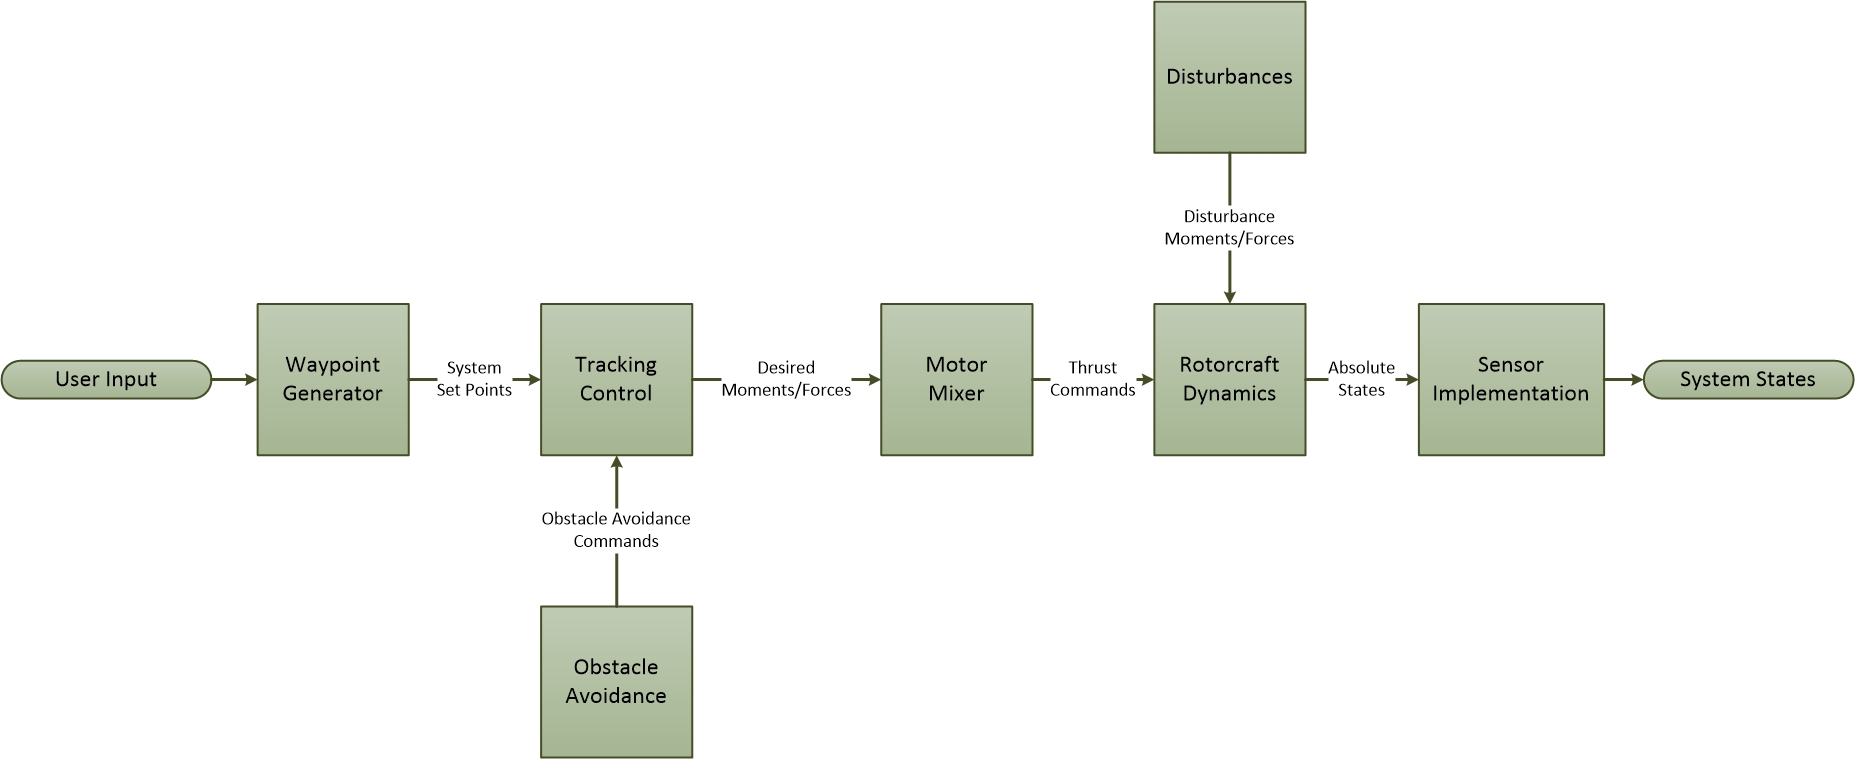
\includegraphics[height = 6cm]{../References/Diagrams/Simulation.jpg} 
		\caption{High level view of simulation set up.}
		\label{IM_Sim}
		\end{figure}
		
	\section{Aims and Objectives}
	The objective of this work was to design an aerial vehicle that is capable of flight inside a confined space and narrow corridor. The first goal is to create a craft that is stable in the presence of system and sensor noise and impurities. The craft must be shown to to perform this task in the presence of disturbances. Once the craft is shown to produce stable results in the presence of disturbances using the designed flight controllers, the obstacle avoidance system needs to be tested. The first test must prove that in a simple environment with disturbances the system remains stable and ensures there is no collision. The next test must be to evaluate the drone navigating in a simple environment with the assistance of the obstacle avoidance controller. The difference with these tests will be to prove that the obstacle avoidance routine will navigate around obstacles and not simply just avoid them. After the drone can successfully navigate a simple environment, a more complex environment needs to be tested creating the needs for more complex manoeuvres. Finally the limitations in the proposed method need to be shown, an environment where the craft will not be able to complete it's desired mission must be shown to understand where improvements and future work can be aimed.

	\section{Testing Methodology and Results}
	This section describes the method and results used to achieve the testing aims outlined above. A multitude of test scenarios are generated, all with a specific purpose to achieve one of the testing aims described above. The testing is structured to follow a logical pattern of validations.
	
		\subsection{Fully Integrated and Controlled System}
		The objective of the first test is to validate the designed controllers in the presence of a large disturbance. The disturbance is simulated as a $5\pm1$\,m/s wind flowing at $45$\textdegree$\pm10$\textdegree, measured off the North axis in a counter clockwise direction. Figures \ref{IM_Test01} and \ref{IM_Test02} are basic step responses with the above mentioned disturbance. The angle of the wind is in the same direction as the East position reference and the opposite direction to the North position reference. The green line in both images depicts the undisturbed system, with the blue line showing the disturbed system.
		
		\begin{figure}[H]
			\centering
			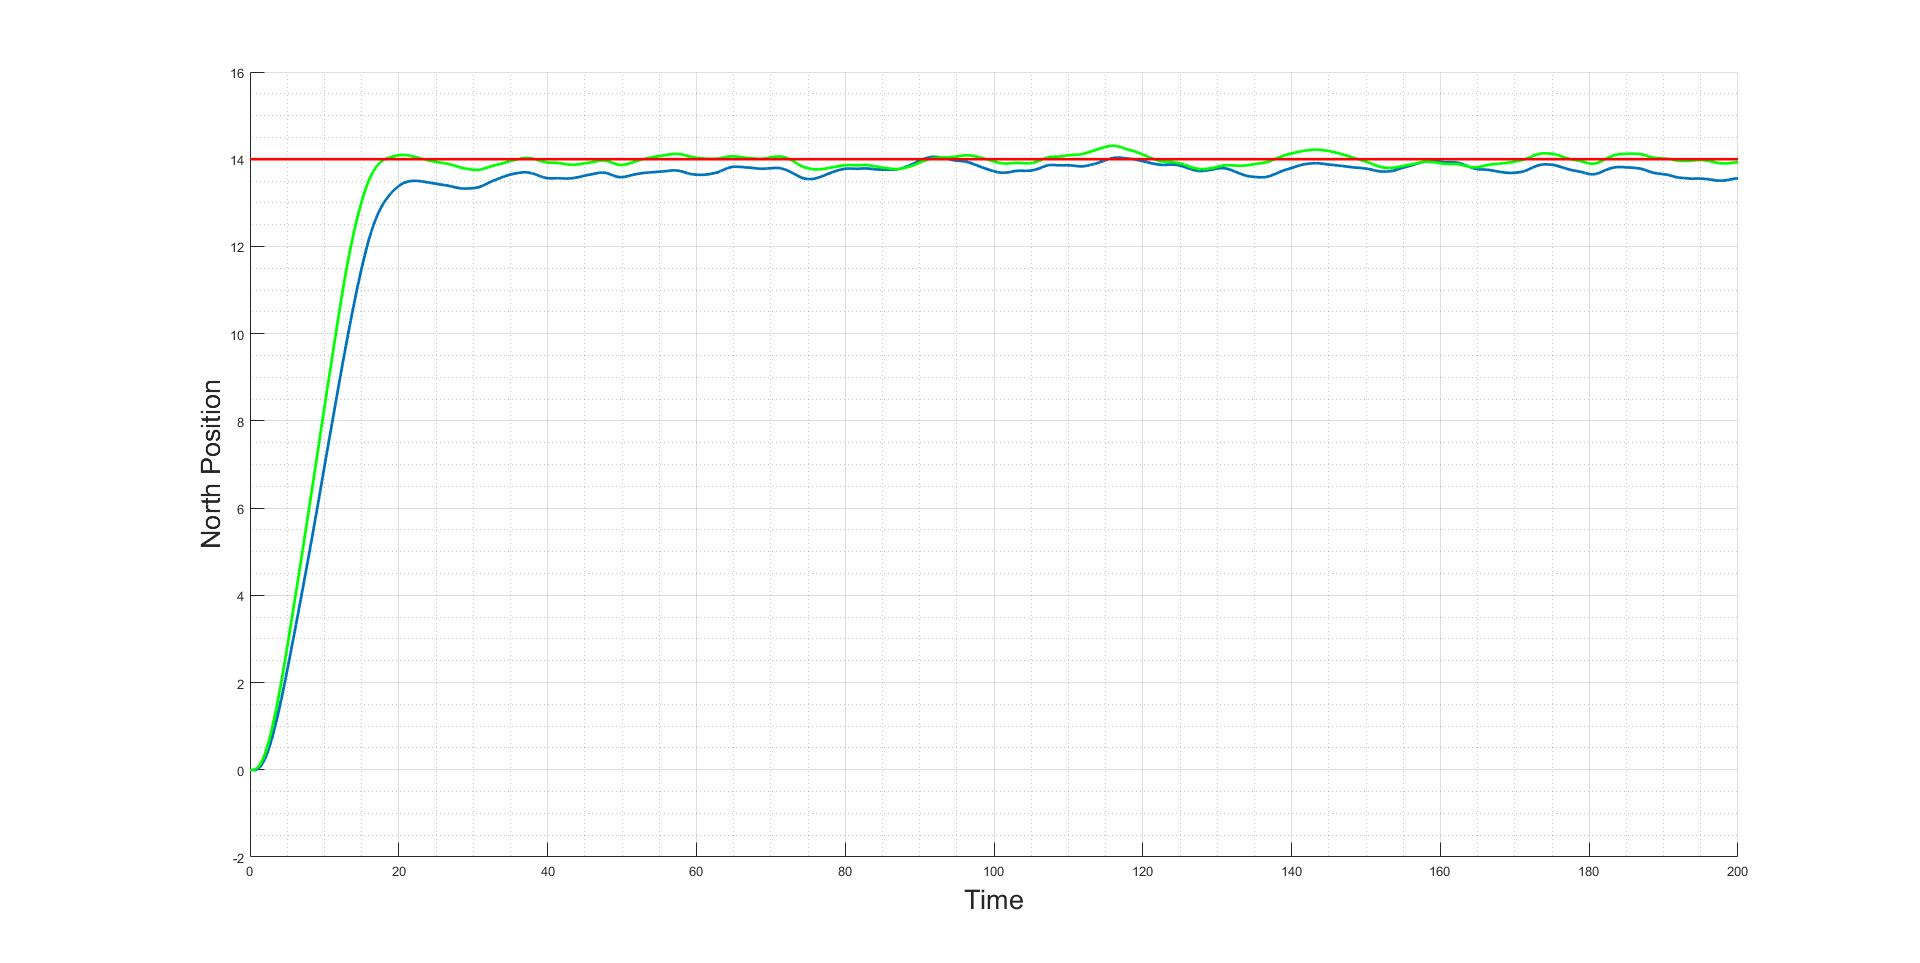
\includegraphics[height = 8cm]{../References/Testing/SimpleWaypoint_Both_North.jpg}     
			\caption{Step response with disturbance - north position plot}
			\label{IM_Test01}
		\end{figure}
		
		\begin{figure}[H]
			\centering
			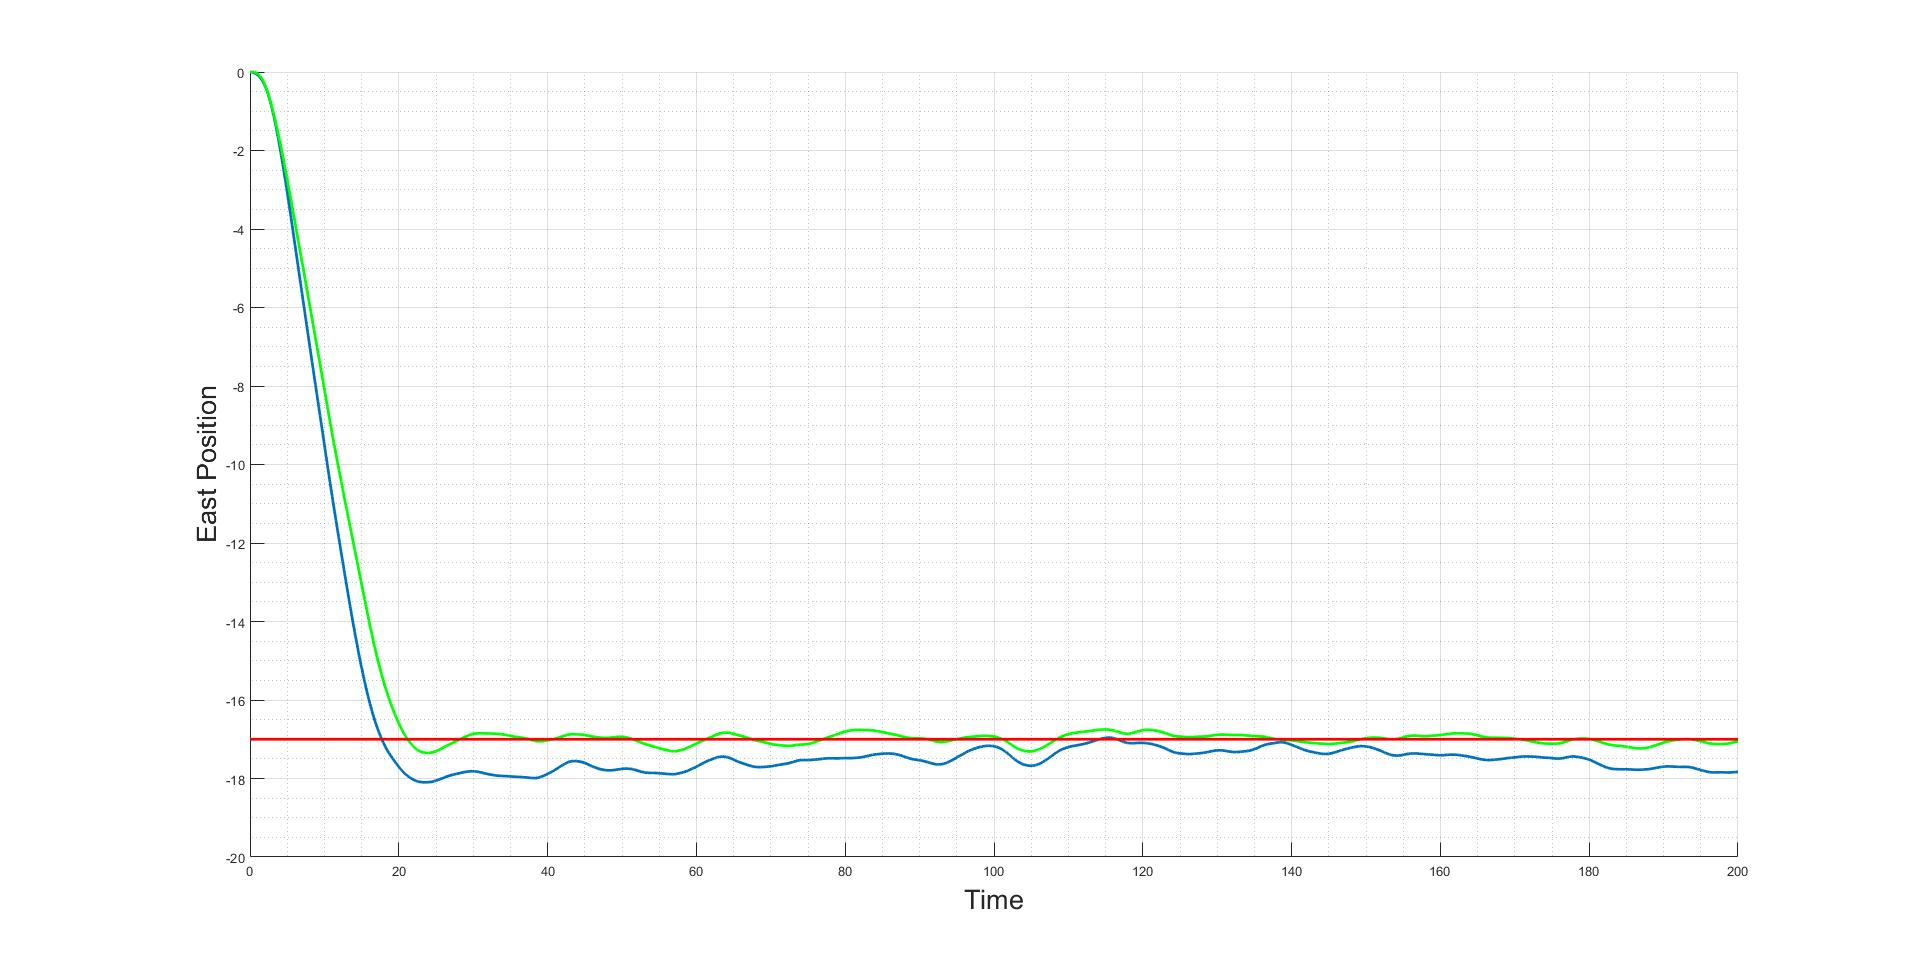
\includegraphics[height = 8cm]{../References/Testing/SimpleWaypoint_Both_East.jpg}     
			\caption{Step response with disturbance - east position plot}
			\label{IM_Test02}
		\end{figure}
		
		The wind causes the East controller to overshoot and sit around $1$\,m off the desired setpoint. The North controller is expected to fly into the wind and as expected exhibits a slower rise time to the non disturbed system.
				
		Next, the waypoint generator is loaded with five waypoints, commanding the drone to first reach a set height and then fly in a rectangle ending at the start point. The large wind is angled to push the drone South and West and is present from the beginning of the simulation. As the craft reaches it's set height the craft is commanded to maintain in it's current North and East position. The North and East controllers will have a small position error until the wind forces the drone off of the set point. An initial offset is thus expected before the velocity controllers are given larger setpoint to follow. Figures \ref{IM_Test11} and \ref{IM_Test12} show the North and East positions respectively.
		
		\begin{figure}[H]
			\centering
			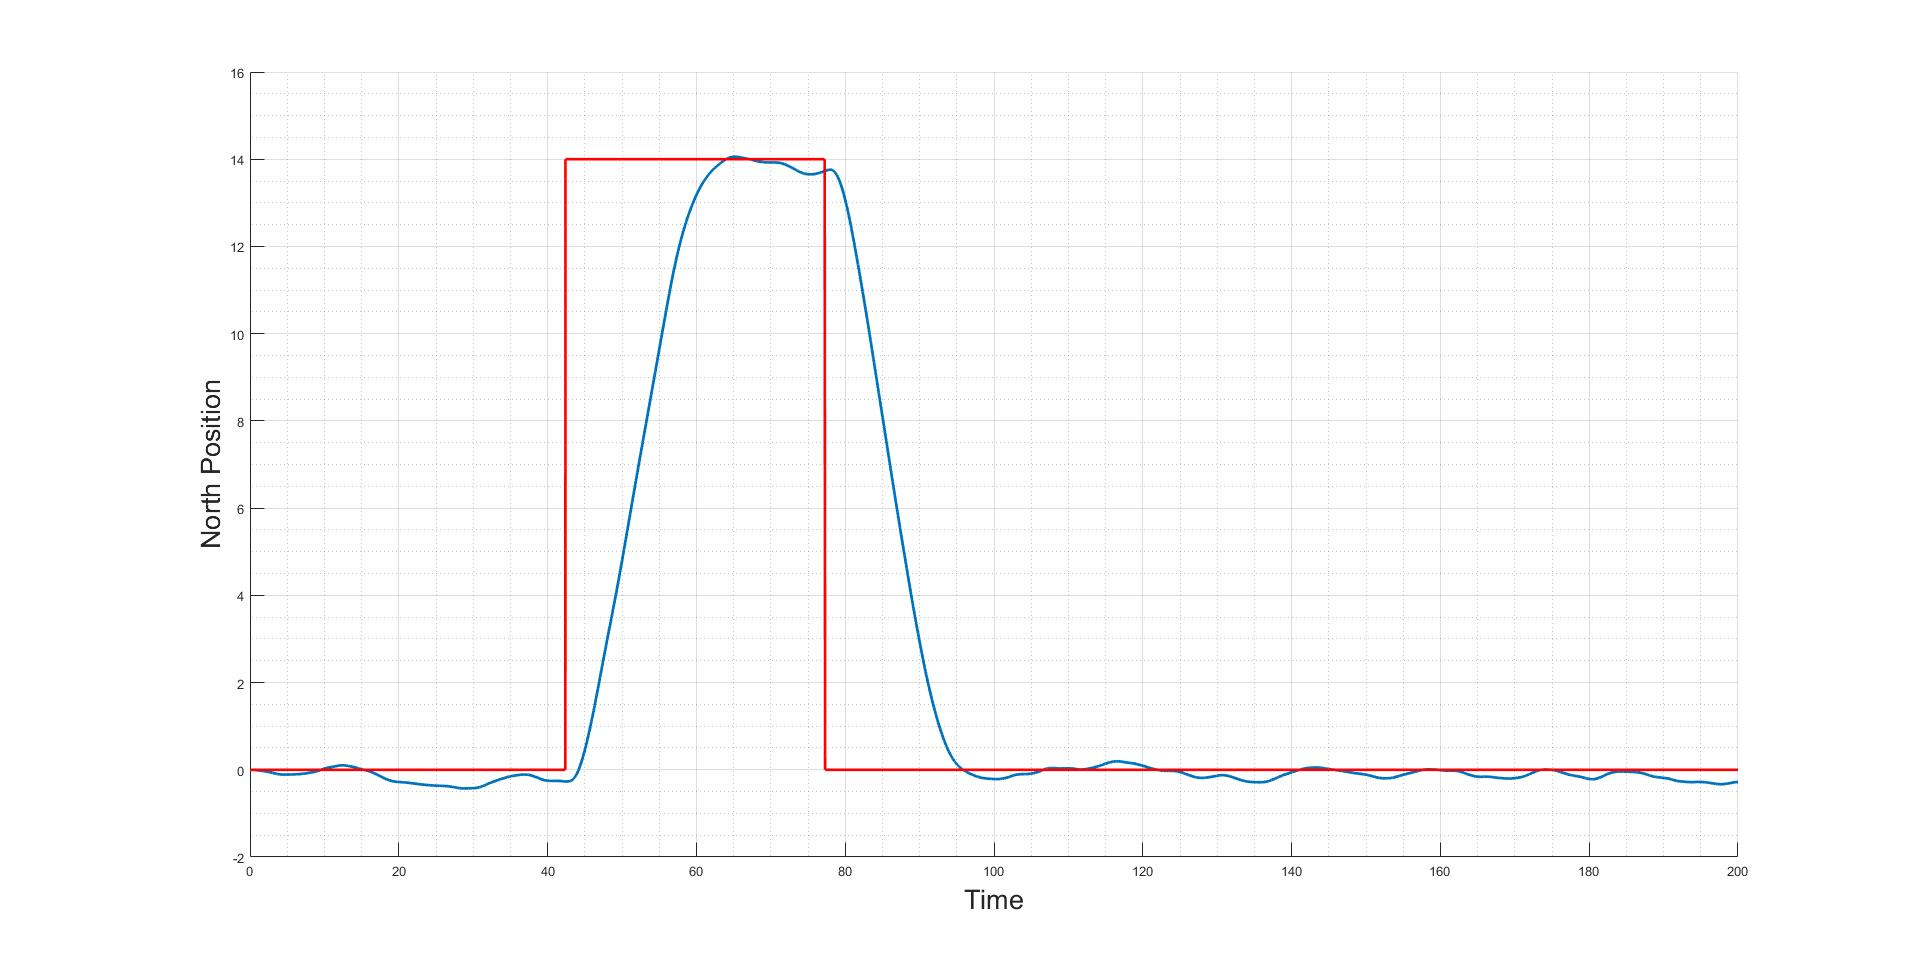
\includegraphics[height = 8cm]{../References/Testing/SimpleWaypoint_5Wind_North.jpg}     
			\caption{Waypoint flight with disturbance - north position plot}
			\label{IM_Test11}
		\end{figure}
		
		The North position is initially offset by the wind and is commanded to fly against the wind before returning South with the wind pushing it towards the setpoint. The North position reaches within $0.5$\,m in both cases. The seemingly linear portion of the curve entails that the disturbance is causing the drone to hit the upper saturation limit of the velocity command.
		
		\begin{figure}[H]
			\centering
			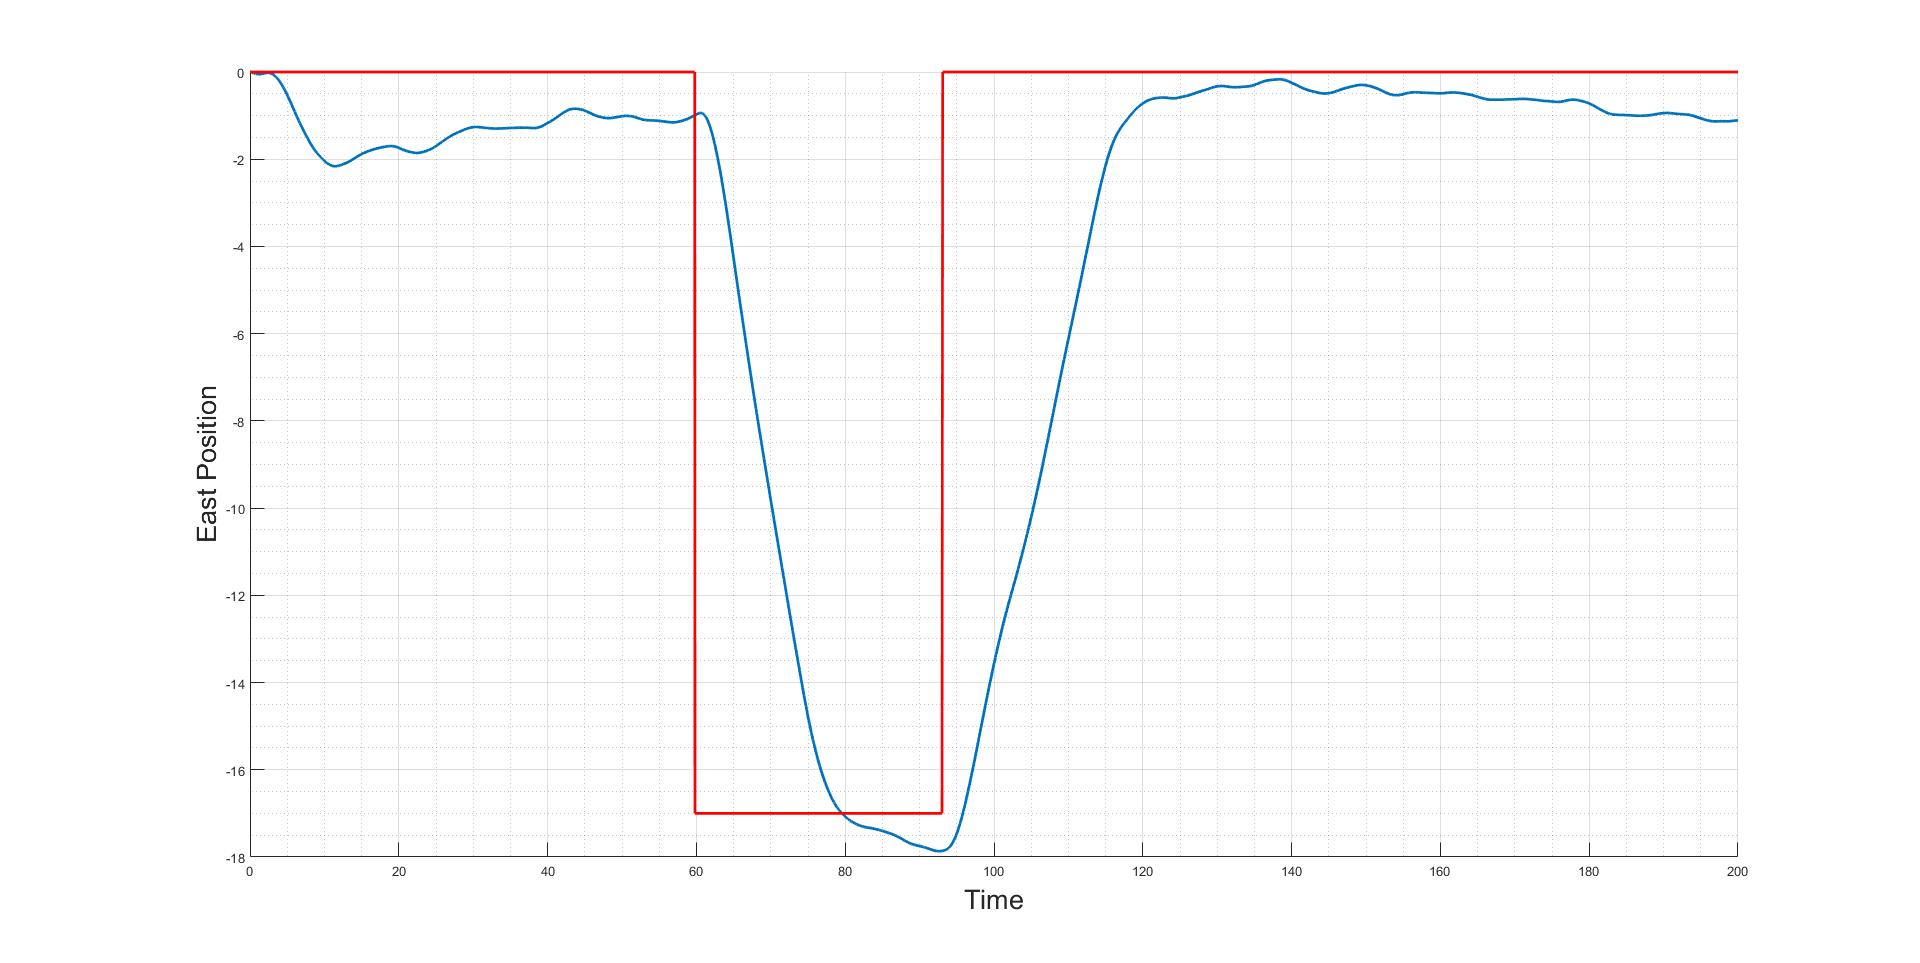
\includegraphics[height = 8cm]{../References/Testing/SimpleWaypoint_5Wind_East.jpg}     
			\caption{Waypoint flight with disturbance - east position plot}
			\label{IM_Test12}
		\end{figure}
		
		The East position has more difficulty handling the disturbance. The non symmetry of the craft causes a larger surface area in that plane, which leads to a larger drag caused by wind disturbances. The East position is intially pushed a maximum of $1.5$\,m off of it's setpoint and settles to just less than a metre off the final desired position.
		
		The above tests show the craft to be stable under simulated disturbances. The craft has more difficulty rejecting disturbances caused by wind in the Y-Body frame of the craft and can be reduced by angling the craft towards the wind during flight.
					
		\subsection{Basic Obstacle Avoidance Routine}
		The next test is designed to evaluate the effectiveness of the obstacle avoidance routine in the presence of a disturbance. The Y-Body Axis was seen to be less resilient towards disturbances and will be tested for this purpose. The test is designed to see if the craft can maintain a set distance away from a wall while the tracking system and disturbance push it towards the wall.
		
		To accomplish a wall was placed along $1$\,m East and another wall at $-3$\,m East as shown by the red lines in Figure \ref{IM_Test21}. A constant $10$\,km/h wind was applied to the craft facing due East, pushing the craft into the wall. The Cyan Dot in the image represents the waypoint at (15, 0). There are two images in Figure \ref{IM_Test21}, the image on the left shows the flown flight path, while the image on the right adds the obstacle avoidance vector generated by the obstacle avoidance controller.
		
		\begin{figure}[H]
			\centering
			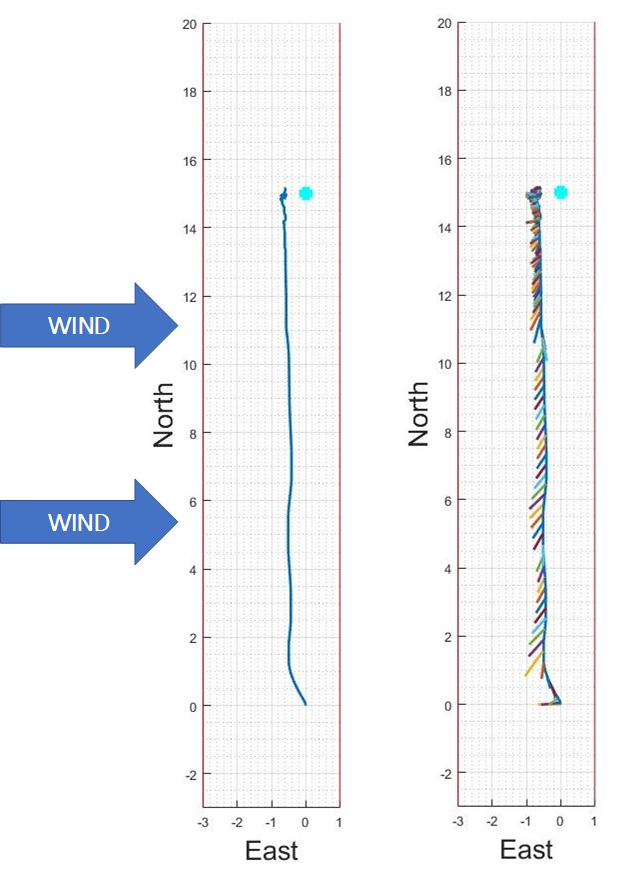
\includegraphics[height = 10cm]{../References/Testing/CorridorFlight_2Wind.jpg}     
			\caption{Corridor flight with disturbance - showing flight path (left) and obstacle avoidance vector (right)}
			\label{IM_Test21}
		\end{figure}
		
		The drone is commanded to position 0 East and the wind is attempting to force the Drone directly East as well. The obstacle avoidance vector successfully steers the craft away from the East wall and maintains an average distance of $0.62$\,m off of the wall with a standard deviation of $0.09$\,m. The obstacle avoidance vector shown in the coloured line of the right image shows the direction in which the drone is being pushed by the obstacle avoidance controller. The proximity to the East wall pushes the drone in a Westward direction, with a South facing component. The derivative portion of the controller creates the South facing vector as it moves in a Northerly direction.
		
		Figures \ref{IM_Test22}, \ref{IM_Test23} and \ref{IM_Test24} show the same flight with each position plotted against time. The green line shows the path flown in a scenario where the obstacle avoidance controller is deactivated. The red line is the set point with the blue line being the flown path with obstacle avoidance activated. The black dotted line in the East plot represent the wall at $1$\,m.
		
		\begin{figure}[H]
			\centering
			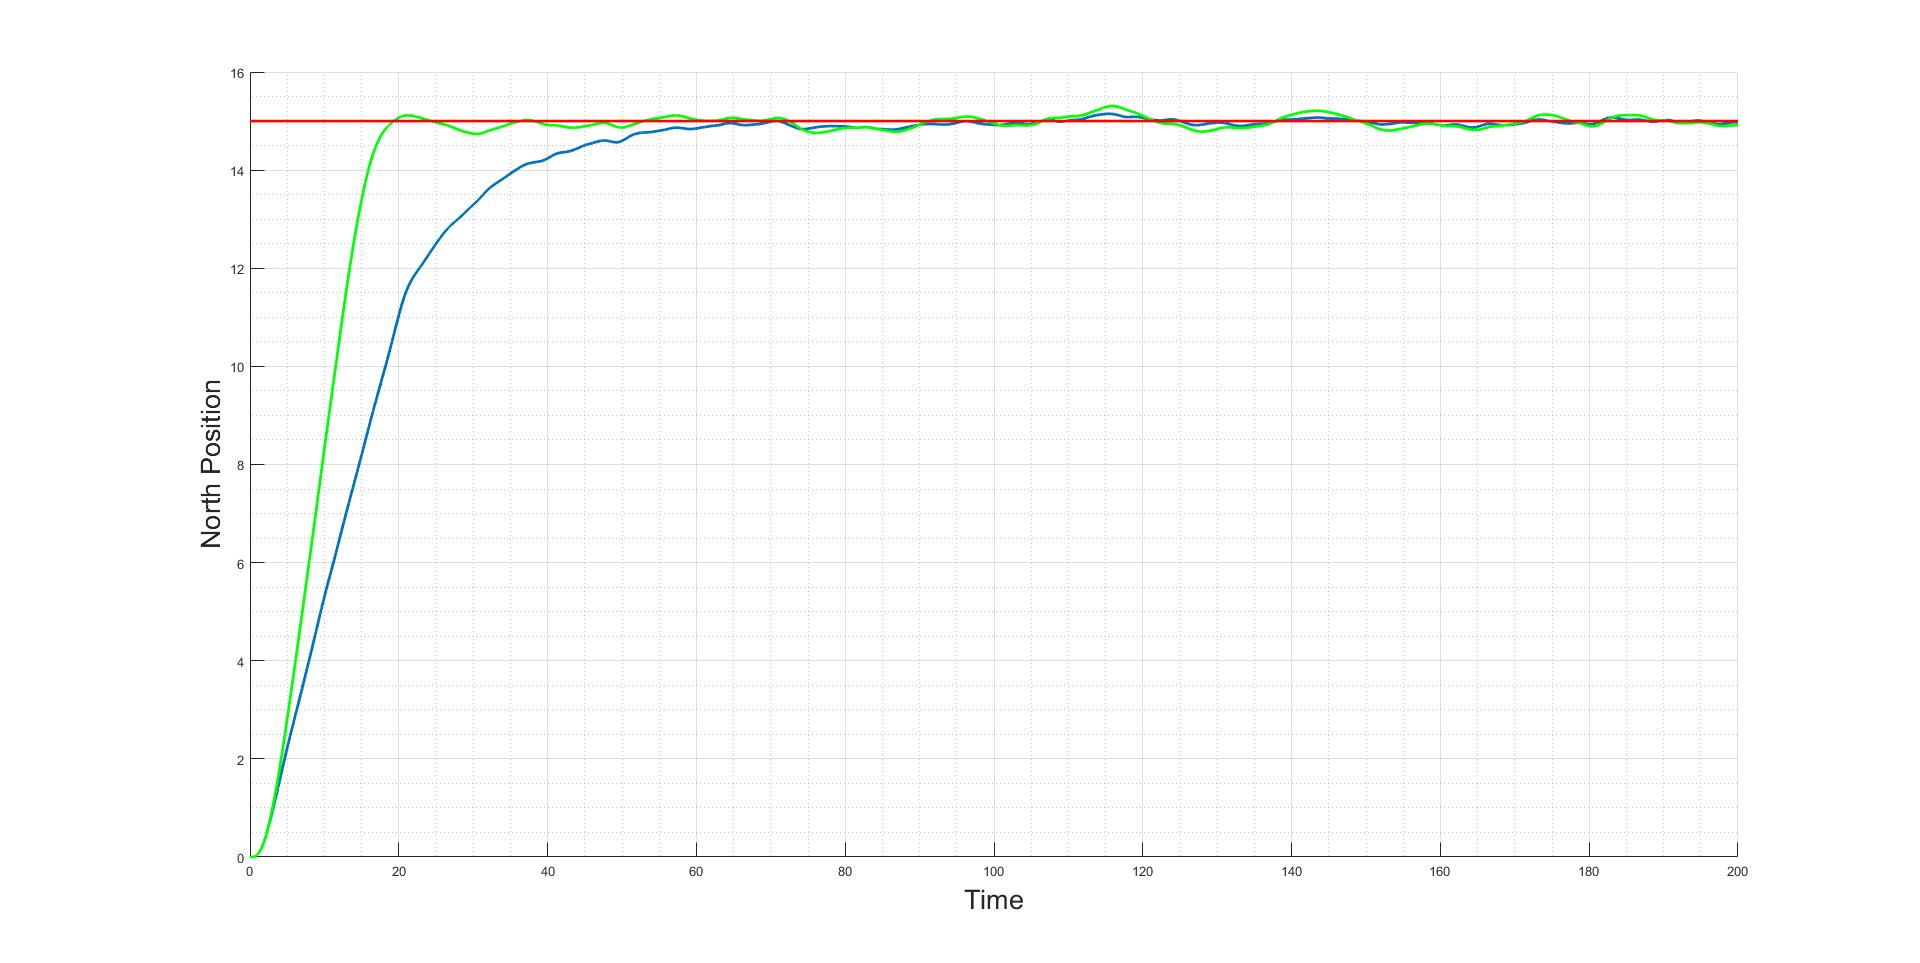
\includegraphics[height = 7.9cm]{../References/Testing/CorridorFlight_2Wind_North.jpg}     
			\caption{Corridor flight with disturbance - north position}
			\label{IM_Test22}
		\end{figure}
		
		The obstacle avoidance controller slows down the North settling time of the craft. The obstacle avoidance controller derivative component will increase damping in the system as seen by the reduced overshoot.
		
		\begin{figure}[H]
			\centering
			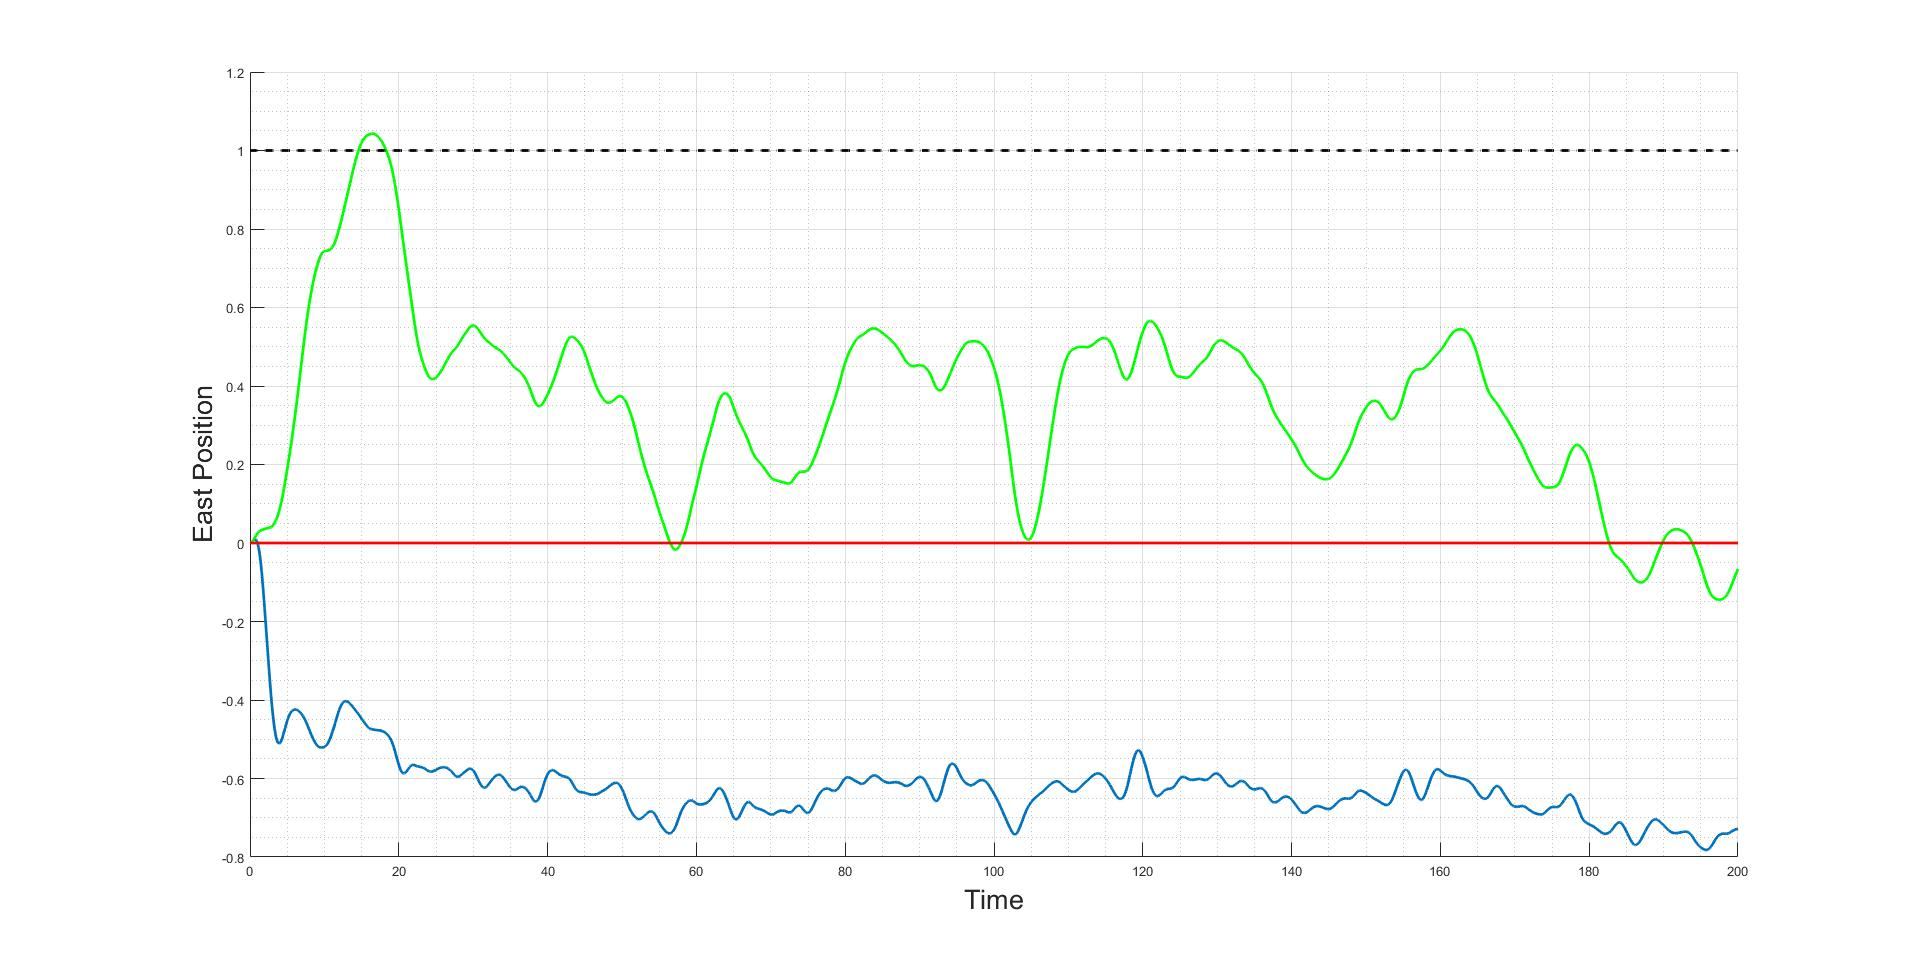
\includegraphics[height = 7.9cm]{../References/Testing/CorridorFlight_2Wind_East.jpg}     
			\caption{Corridor flight with disturbance - east position}
			\label{IM_Test23}
		\end{figure}
		
		As expected from the previous test, without the obstacle avoidance controller the drone will collide with the wall at $1$\,m. The obstacle avoidance controller pushes the craft off of it's setpoint to ensure it maintains a set distance form the wall. The increased damping in the obstacle avoidance controller also reduces the oscillations seen by the craft.
		
		\begin{figure}[H]
			\centering
			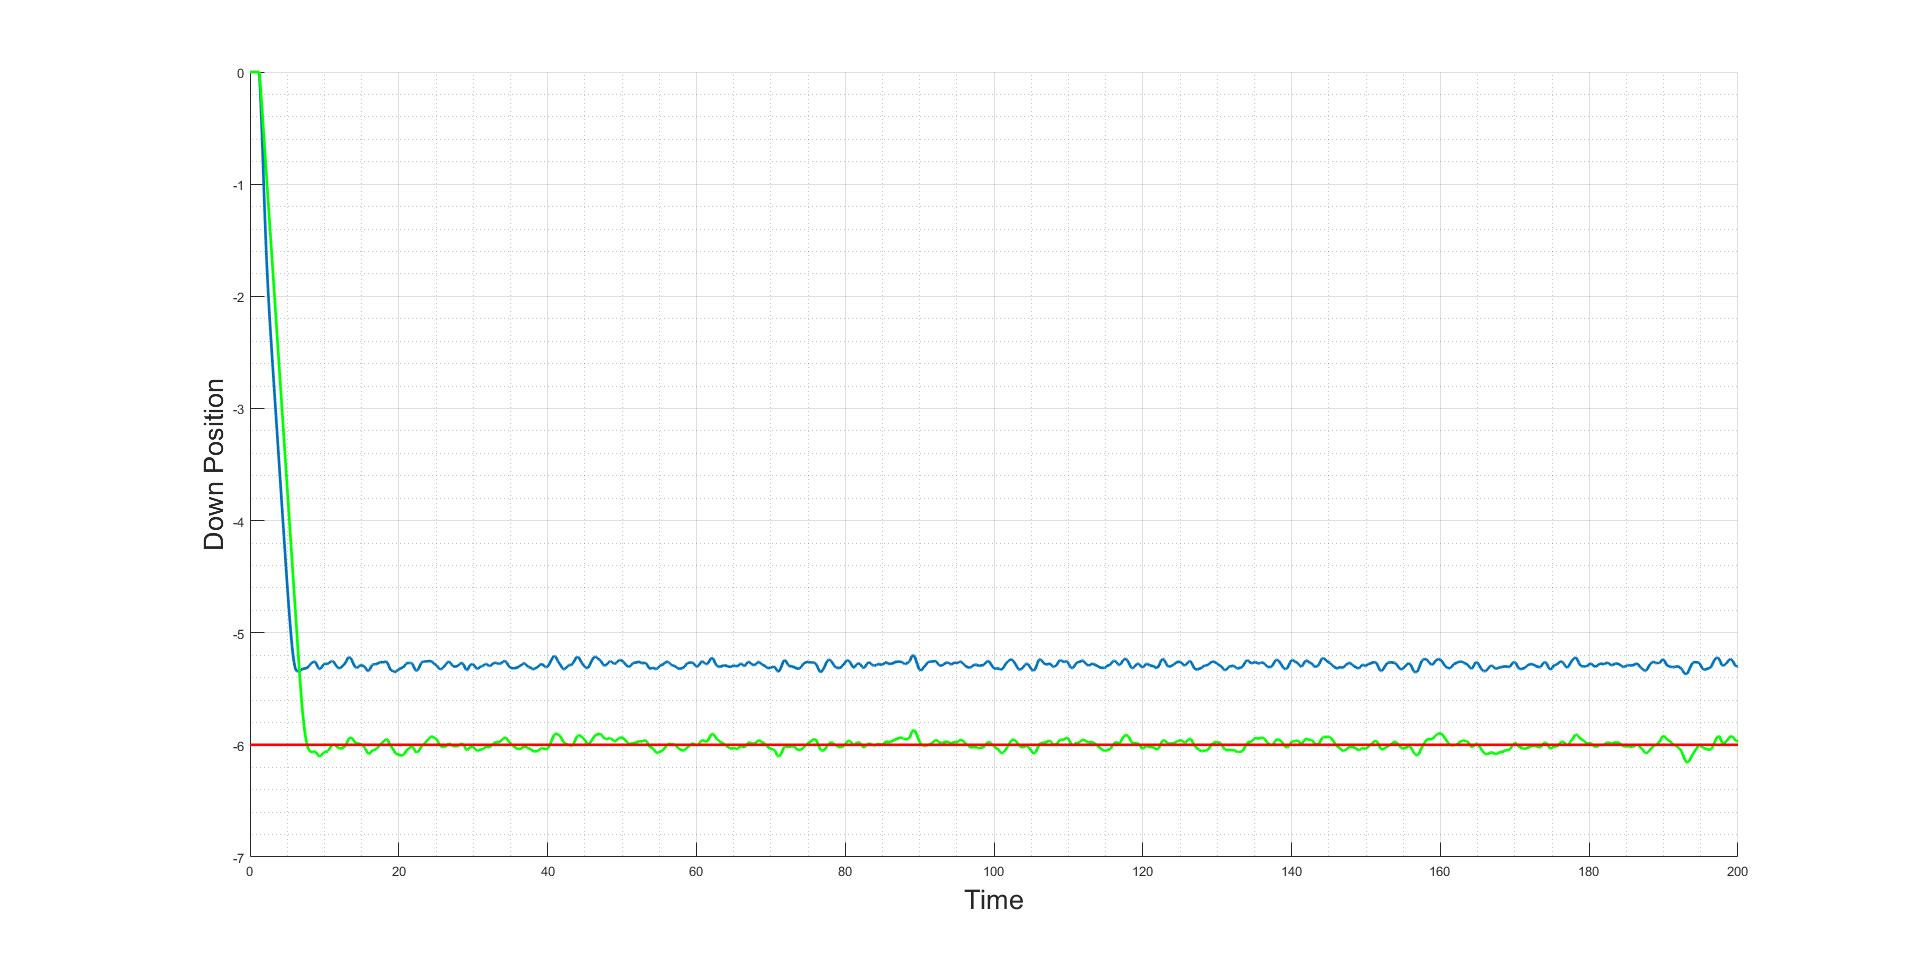
\includegraphics[height = 7.9cm]{../References/Testing/CorridorFlight_2Wind_Down.jpg}     
			\caption{Corridor flight with disturbance - down position}
			\label{IM_Test24}
		\end{figure}
		
		The horizontal obstacle avoidance has been the main focus this far. In this scenario a roof was placed at $6$\,m with a floor at $0$\,m. The craft settles an average distance of $0.71$\,m from the roof with a standard deviation of $0.03$\,m.
		
		The obstacle avoidance system has shown it's effectiveness by avoiding a collision in the presence of a disturbance. The routine successfully kept the drone away from the walls by maintaining a set distance. The routine also ensures that the craft flies slowly and steady when in the presence of obstacles.
		
		\subsection{Obstacle Avoidance Navigation}
		The next series of tests aims to test the capabilities of the obstacle avoidance routine and it's ability to navigate through a simple terrain. To test this different test scenarios have been configured. Each environment is in a sawtooth shape which traverses from South to North. The drone will be given only a North reference with the East position controller disabled. The obstacle avoidance routine will be required to ensure the drone does not collied with any of the walls, as well as find a path through the corridor to the desired North position. The test will be run three times. The first test will be in a wide corridor where the obstacle avoidance sensors will not always be activated. The second test will be a narrow corridor which will show how the craft behaves if it is constantly in close proximity to a wall. The third test will show the effect the yaw alignment algorithm, has on the system and vice versa.
		
			\subsubsection{Wide Corridor}
			The first test requires a large corridor to be used and are represented by the red lines in Figure \ref{IM_Test31}. The vehicle is commanded to fly to a North position of $34$\,m as shown by the cyan line. The flown path is shown in blue with the obstacle avoidance vector shown in the coloured line. The East position control is completely dictated by the obstacle avoidance routine.
			
			\begin{figure}[H]
				\centering
				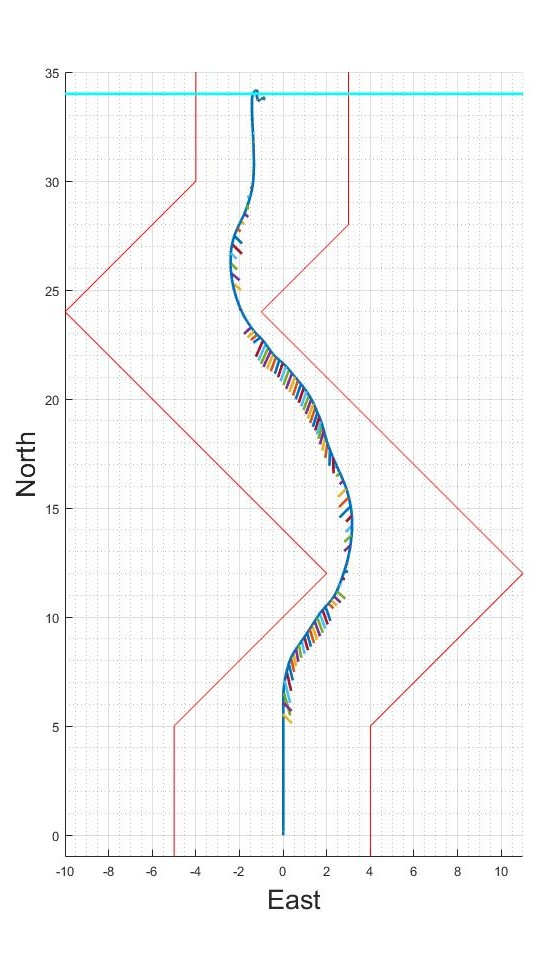
\includegraphics[height = 14cm]{../References/Testing/WideCorridor3DProx.jpg}     
				\caption{Navigated flight in a wide corridor}
				\label{IM_Test31}
			\end{figure}
			
			The craft maintains a minimum distance of $0.5$\,m away from the wall and flies along an efficient path to reach the goal, only deferring from the straight line path when necessary to avoid a wall. Although a successful flight, the image does show the importance of the density for sensor placement. The sharp corners created by the wall only activate one of the sensors which creates a small obstacle avoidance vector. Having a more dense sensor placement will nudge the drone further away from the dangerous corners.
			
			\subsubsection{Narrow Corridor}
			The next tests showcases the drone's ability to fly in a confined space where the obstacle avoidance vector is always activated from multiple sides. The narrow corridor is shown in Figure \ref{IM_Test32}, with the drone requested to reach $17$\,m North. Once again the East position of the craft is completely dictated by the obstacle avoidance vector. The coloured line also once again demonstrates the current obstacle avoidance vector which is commanding velocities.
			
			\begin{figure}[H]
				\centering
				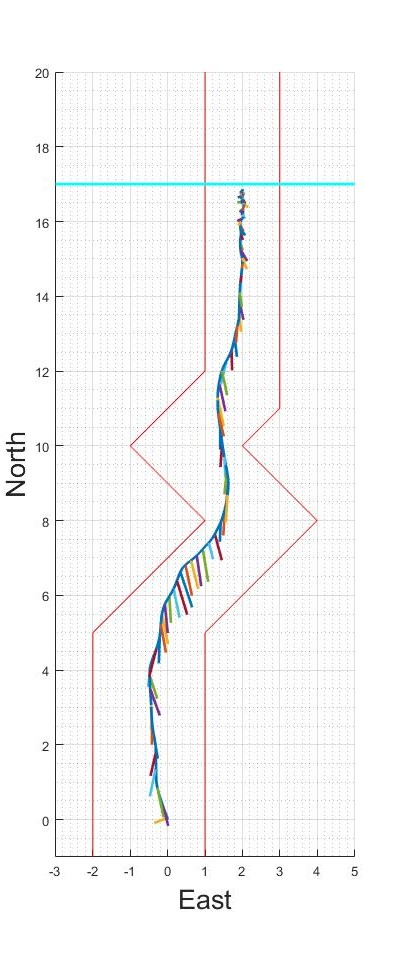
\includegraphics[height = 15cm]{../References/Testing/NarrowCorridor3DProx.jpg}     
				\caption{Navigated flight in a narrow corridor}
				\label{IM_Test32}
			\end{figure}
			
			The drone remains a minimum of $0.5$\,m away from the walls. This test demonstrates the importance of the derivative action of the obstacle avoidance vector, specifically in a confined space. Although all the sensors are active due to close proximity to multiple walls, the walls which the drone is approaching take precedence and the obstacle avoidance controller forces large action. The walls which the drone is not approaching have limited interference for the flight path.
			
			\subsubsection{Yaw Alignment in a Confined Space}
			The next test is designed to evaluate the operation of both the obstacle avoidance and the yaw alignment strategies when used in conjunction with one another. The wide corridor test is run again, this time with the yaw alignment routine activated. Figures \ref{IM_Test33}, \ref{IM_Test34} and \ref{IM_Test35} represent the results from those flights. The first image shows only the flown path with the second image including the heading vector of the craft.
			
			\begin{figure}[H]
				\centering
				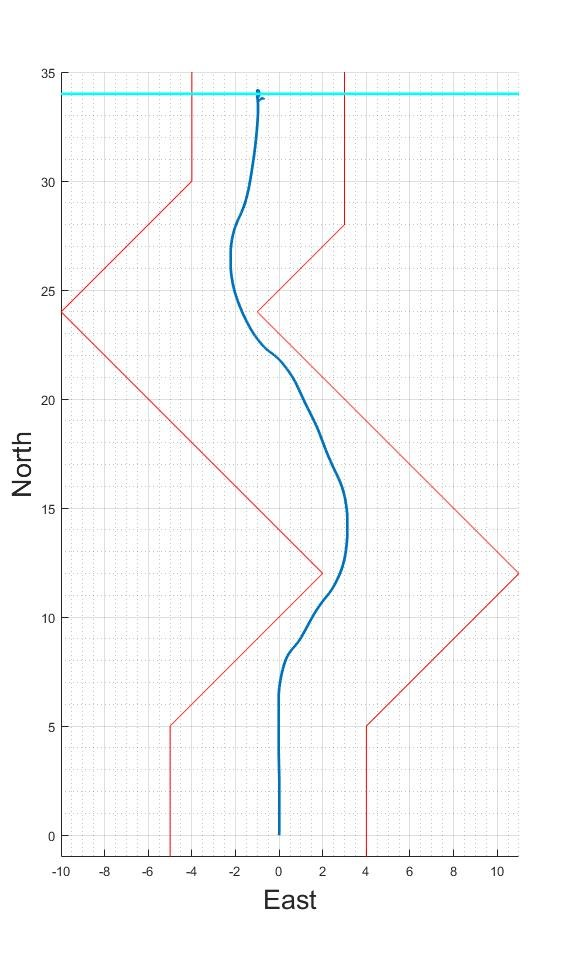
\includegraphics[height = 10cm]{../References/Testing/WideCorridorYawAlign3D.jpg}     
				\caption{Navigated flight in wide corridor with yaw alignment}
				\label{IM_Test33}
			\end{figure}
			
			The path flown closely resembles that of the original path without yaw alignment. The craft does however get closer to the sharp corners of the wall, the yawing craft will affect the response of the obstacle avoidance controller due to the changing sensor readings. A tight sensor placement density will reduce the effect this has on the craft.
			
			\begin{figure}[H]
				\centering
				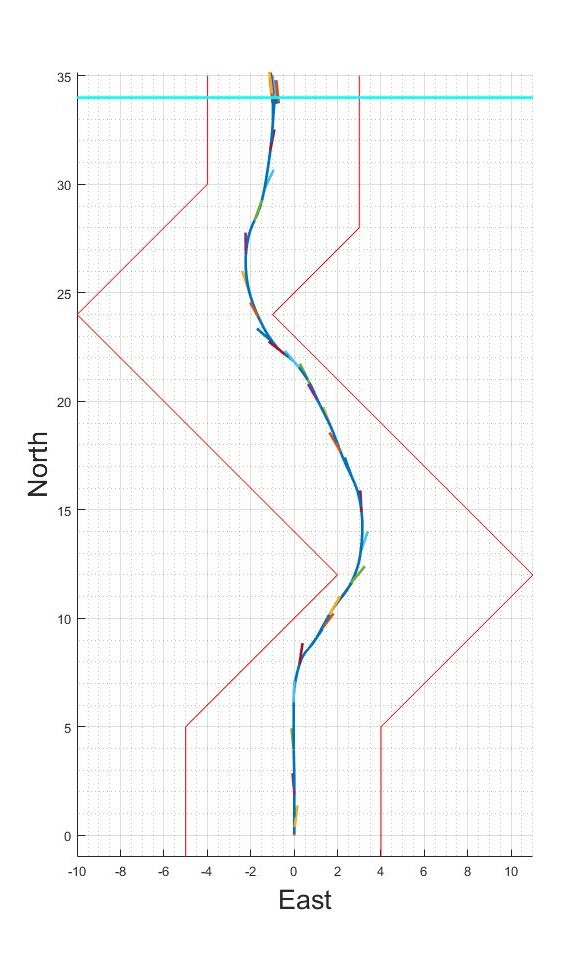
\includegraphics[height = 10cm]{../References/Testing/WideCorridorYawAlign3DAlign.jpg}     
				\caption{Navigated flight in wide corridor with yaw alignment showing current heading of craft}
				\label{IM_Test34}
			\end{figure}
			
			Figure \ref{IM_Test34} overlays the current heading of the craft on the flight path. The yaw alignment is shown to work reasonably well but can be quantified better using Figure \ref{IM_Test35} which shows the yaw error throughout the flight.
			
			\begin{figure}[H]
				\centering
				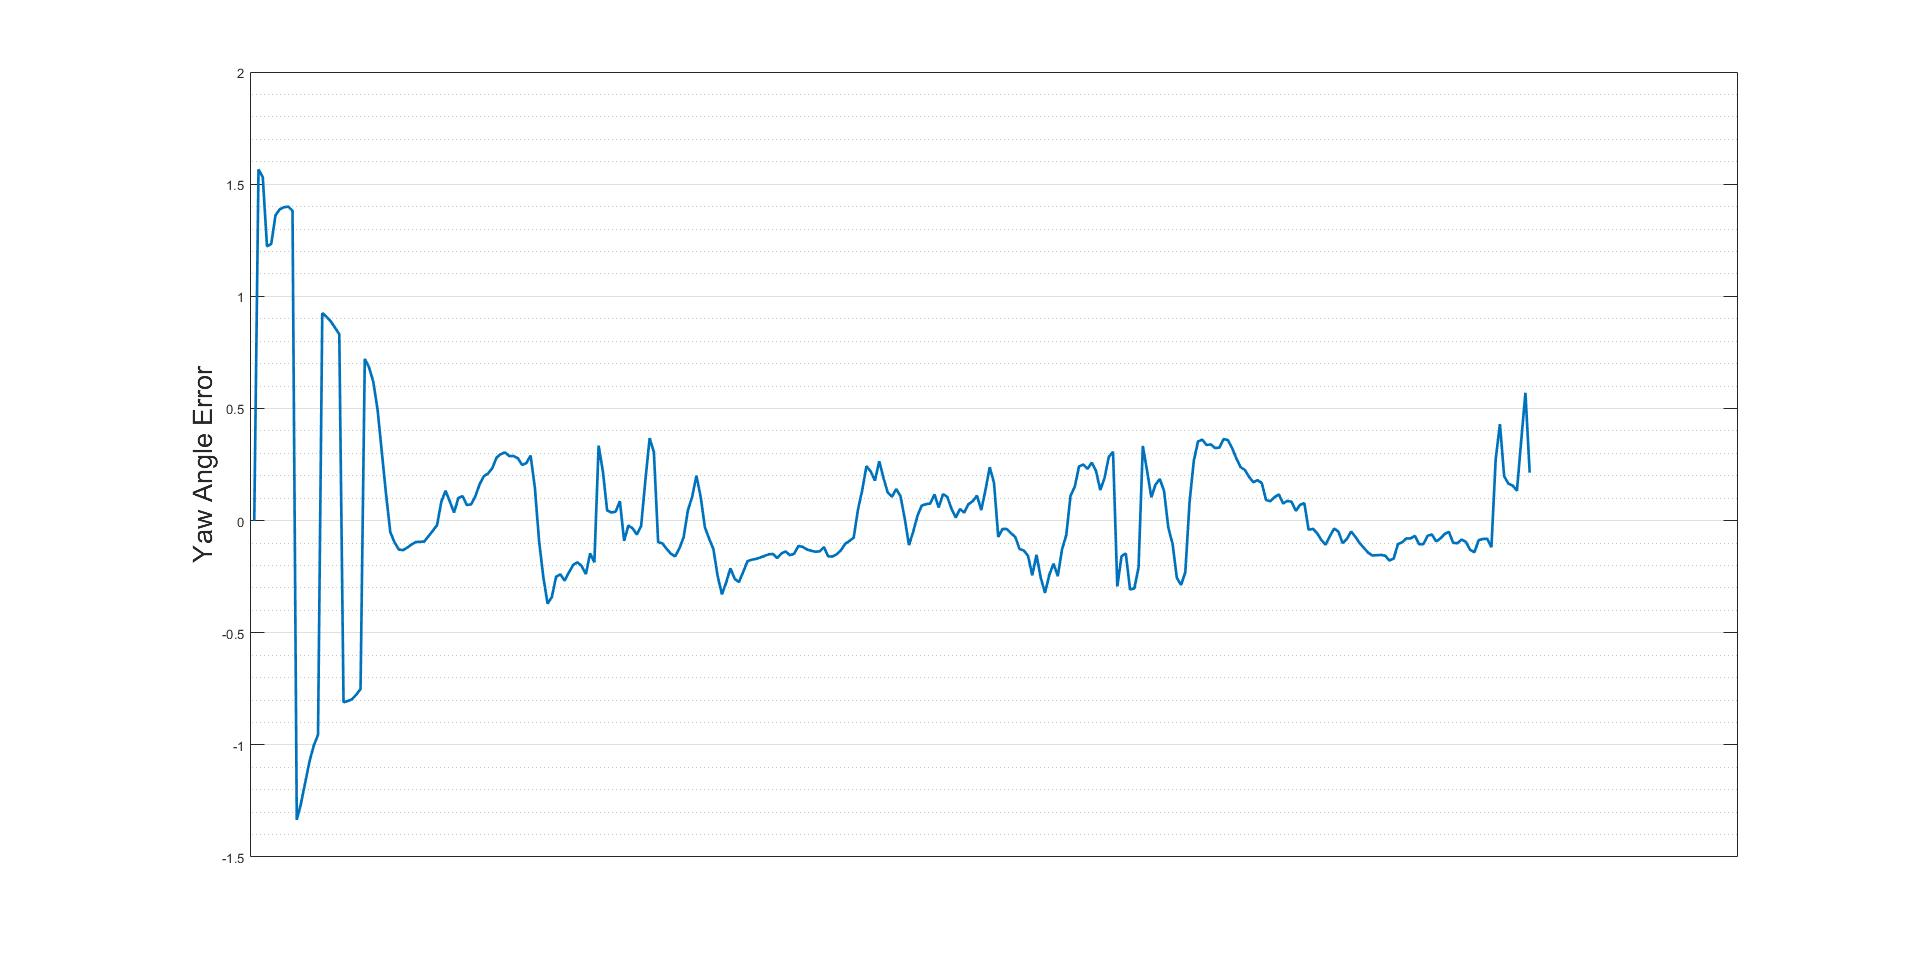
\includegraphics[height = 7.9cm]{../References/Testing/WideCorridorYawAlignYawError.jpg}     
				\caption{Yaw error of vehicle during navigated flight in wide corridor with yaw alignment}
				\label{IM_Test35}
			\end{figure}
			
			The yaw alignment routine runs at a slower pace to that of the velocity controller and hence has large error when there is a sudden change of direction. The average yaw alignment error for the flight is only $1.97$\textdegree with a large standard deviation of $21.53$\textdegree. The constant changes of the craft's velocity leads to varying alignment reference which can cause to a large deviation in error measurements. In some mission cases this might be unacceptable and the craft's current velocity should not be used as the alignment vector, but rather a set heading which can be varied.
		
		\subsection{Generic Mission Flight}
		Now that each component of the craft's control system has been tested and verified a generic example of flight test can be created. This group of tests is run in a simulated environment that contains a combination of open spaces, narrow corridors and unexpected obstacles. The waypoint generator is loaded with 9 waypoints loosely placed around the environment. The waypoints are placed to designed to make the craft explore the entire environment with the need for avoiding obstacles and flying down corridors un assisted. The final waypoint is placed in an unavailable location to assess the craft's behaviour. The test is run both with and without the yaw alignment routine enabled.
		
		The images seen in Figure \ref{IM_GenTest} show both runs with and without their proximity vectors. The waypoints are shown in cyan, starting at (0, 0) and moving in a counter clockwise direction. The last waypoint is placed inside the wall where the drone cannot fly. 
		
		\begin{figure}[H]
			\begin{tabular}{c c}
				\centering
				{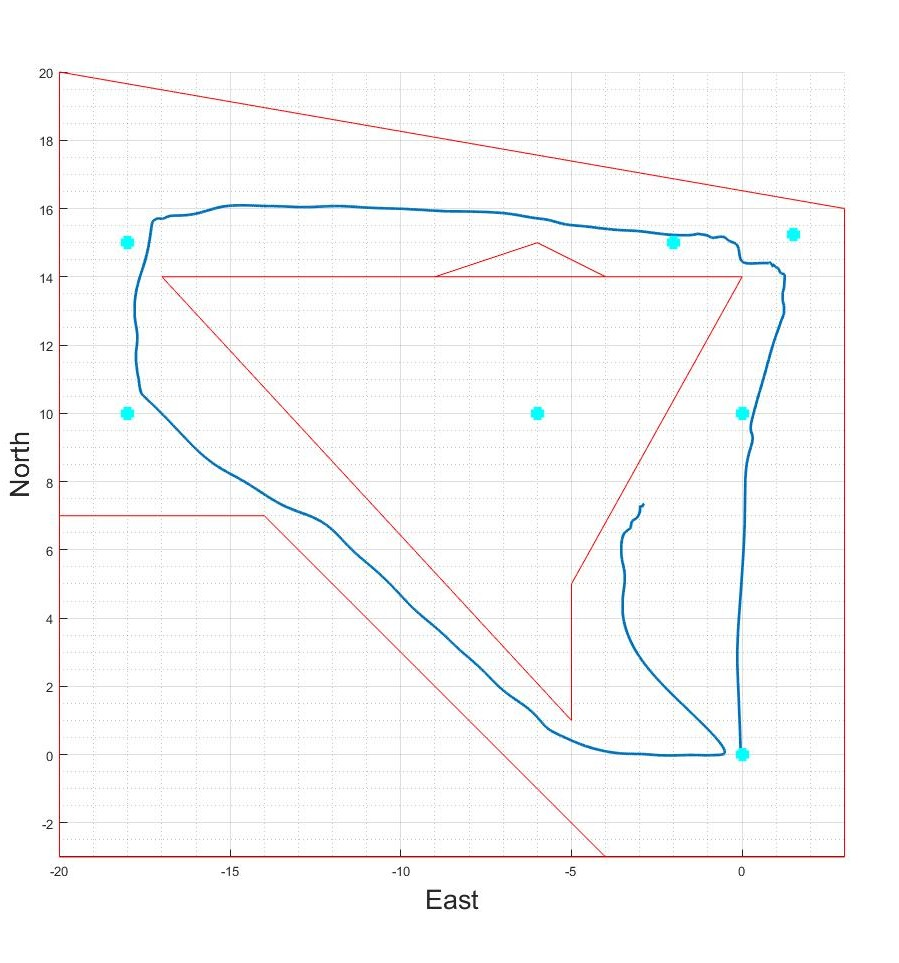
\includegraphics[width = 3in]{../References/Testing/FullRun.jpg}} &
				{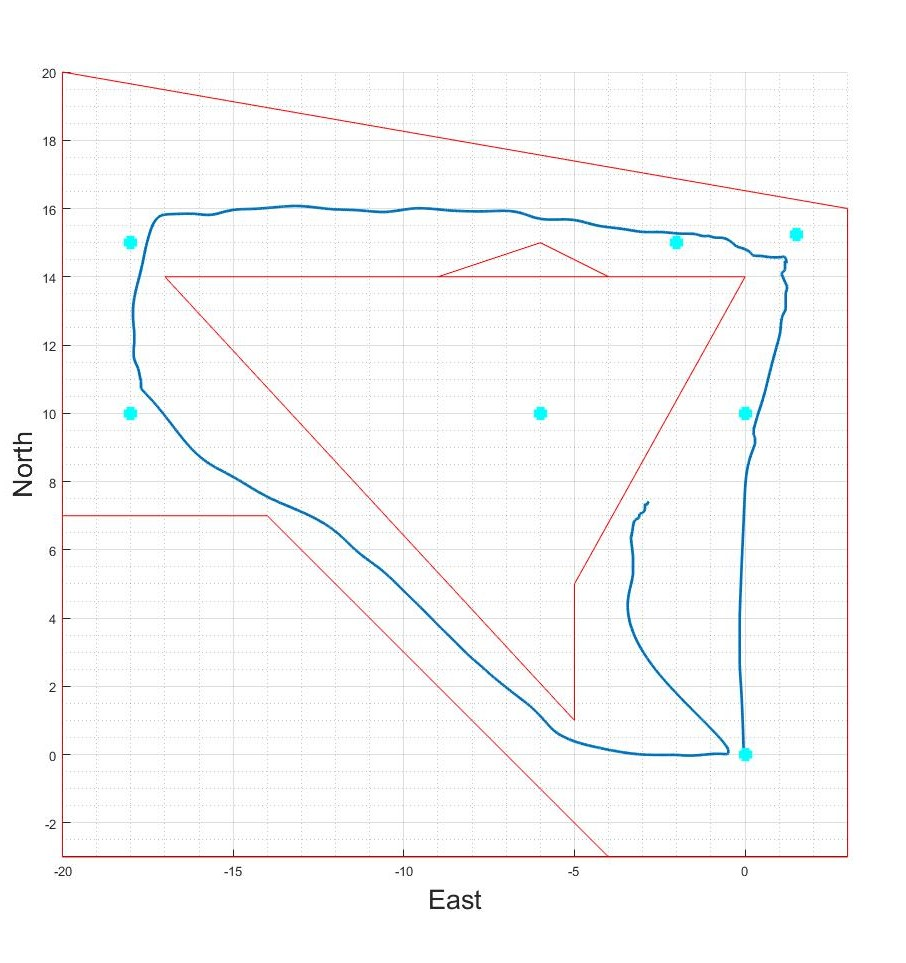
\includegraphics[width = 3in]{../References/Testing/FullRunAlign.jpg}}\\
				{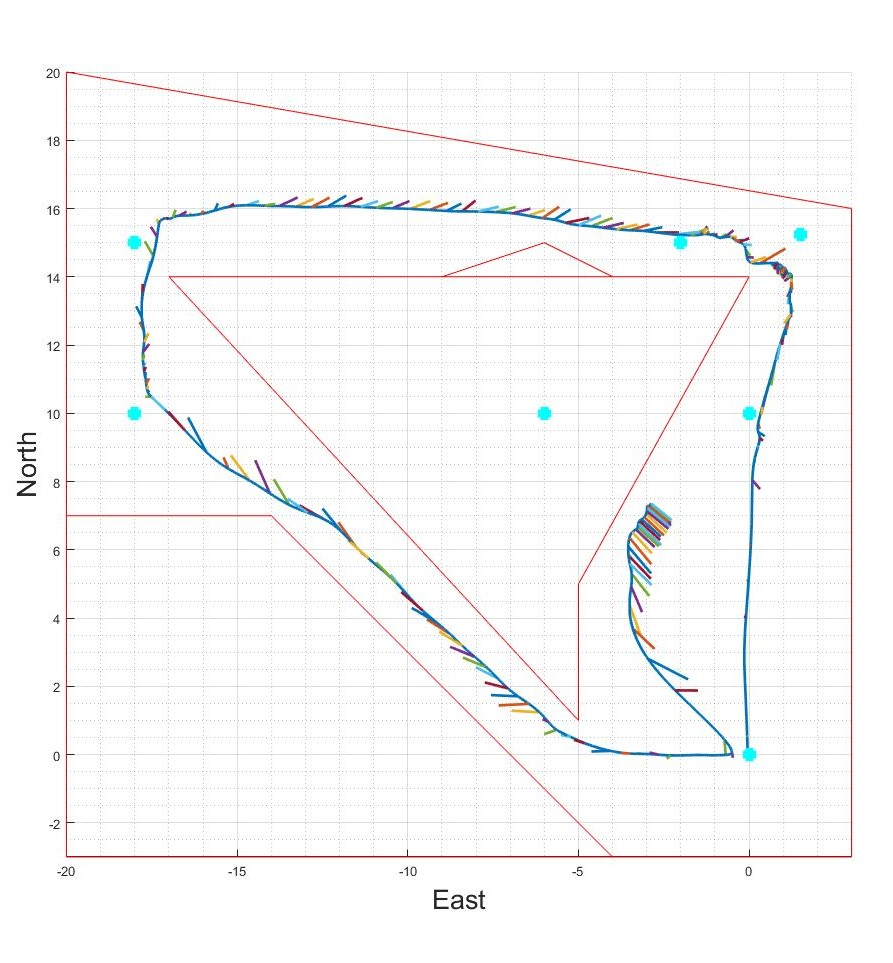
\includegraphics[width = 3in]{../References/Testing/FullRunProx.jpg}} &
				{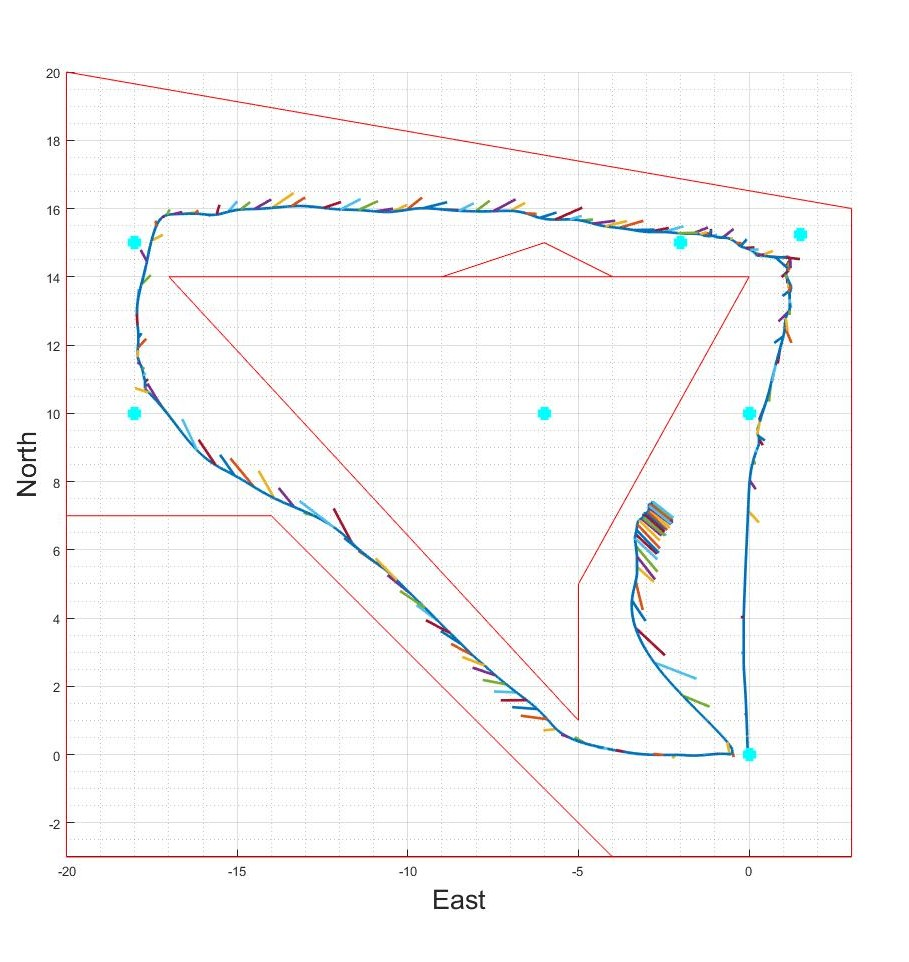
\includegraphics[width = 3in]{../References/Testing/FullRunAlignProx.jpg}}\\
			\end{tabular}
			\caption{Generic mission flight in a simulated environment with loosely placed waypoints. (Left - no yaw alignment, Right - yaw alignment)}
			\label{IM_GenTest}
		\end{figure}
		
		The craft does not hit any obstacles in both runs. A more detailed flight path or a more dense sensor placement would assist in ensuring the craft keeps a further proximity from the sharp corners.
		
%%		\texttt{\begin{figure}[H]
%%			\centering
%%			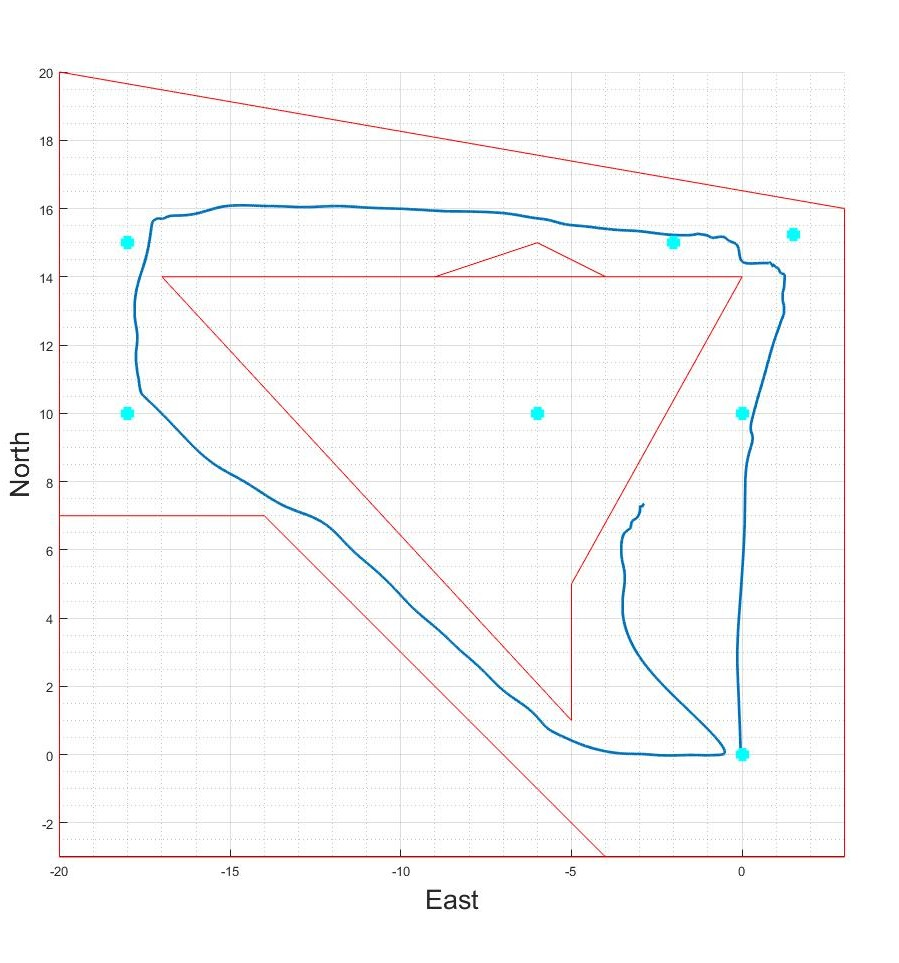
\includegraphics[height = 10cm]{../References/Testing/FullRun.jpg} 
%%			\caption{Navigated Flight in Narrow Corridor}
%%			\label{IM_Test41}
%%		\end{figure}
%%		
%%		\begin{figure}[H]
%%			\centering
%%			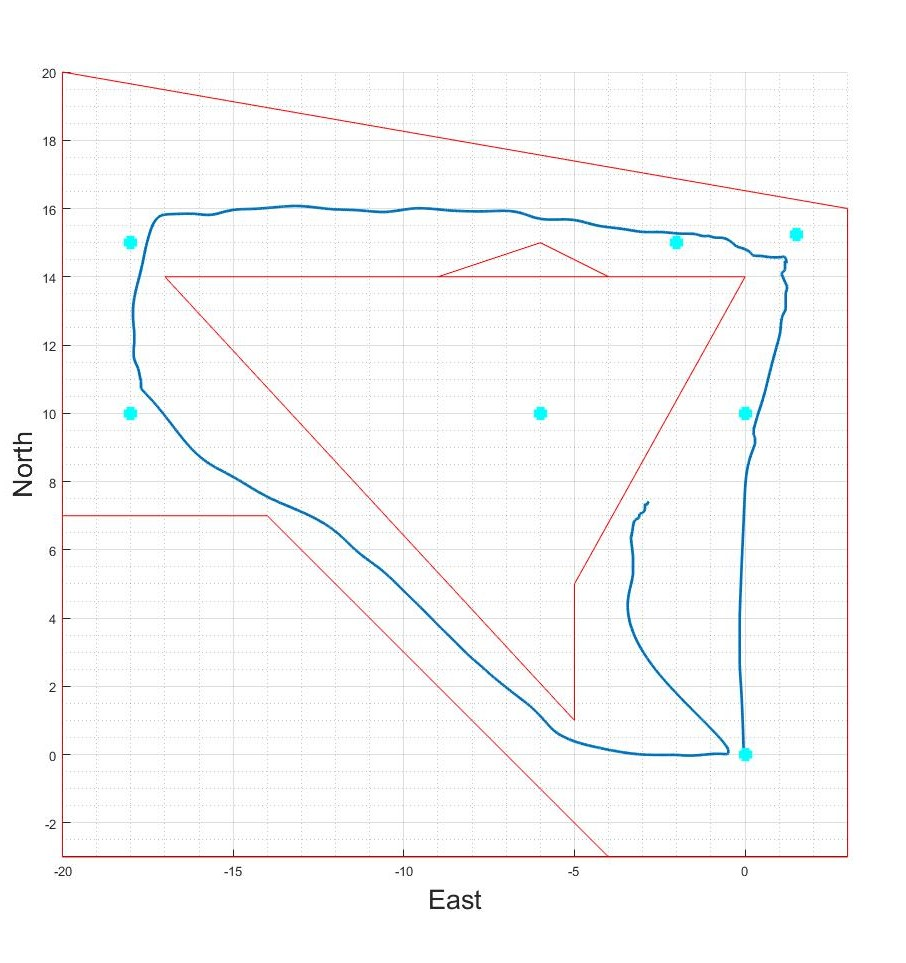
\includegraphics[height = 10cm]{../References/Testing/FullRunAlign.jpg} 
%%			\caption{Navigated Flight in Narrow Corridor}
%%			\label{IM_Test42}
%%		\end{figure}
%%		
%%		\begin{figure}[H]
%%			\centering
%%			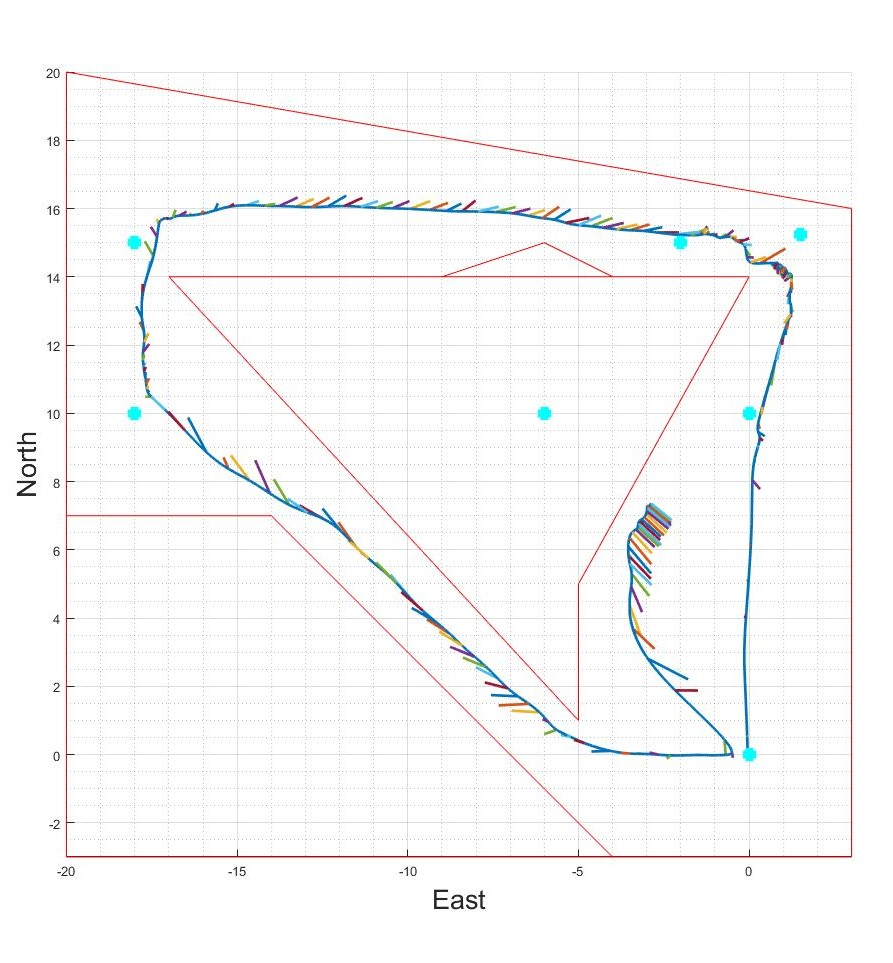
\includegraphics[height = 10cm]{../References/Testing/FullRunProx.jpg} 
%%			\caption{Navigated Flight in Narrow Corridor}
%%			\label{IM_Test43}
%%		\end{figure}
%%		
%%		\begin{figure}[H]
%%			\centering
%%			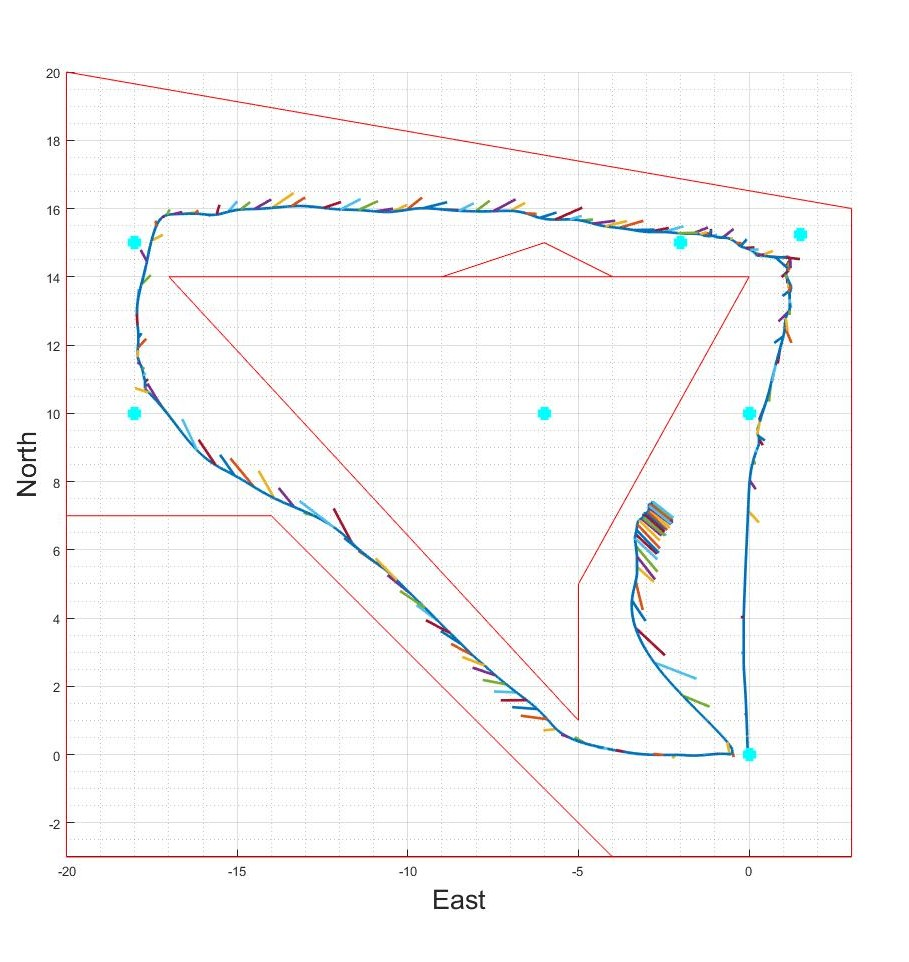
\includegraphics[height = 10cm]{../References/Testing/FullRunAlignProx.jpg} 
%%			\caption{Navigated Flight in Narrow Corridor}
%%			\label{IM_Test44}
%%		\end{figure}}
		
		A better analysis of the separate runs can be made while observing the North and East positions relative to time as shown in Figures \ref{IM_Test46} and \ref{IM_Test47}. The green line shows the position without yaw alignment, while the blue line shows the position when yaw alignment is disabled. The average difference between the position along the North axis is $0.12$\,m with a standard deviation of $0.79$\,m. The East axis boasts a mean difference of only $3$\,cm with a standard deviation of $0.6$\,m.
		
		\begin{figure}[H]
			\centering
			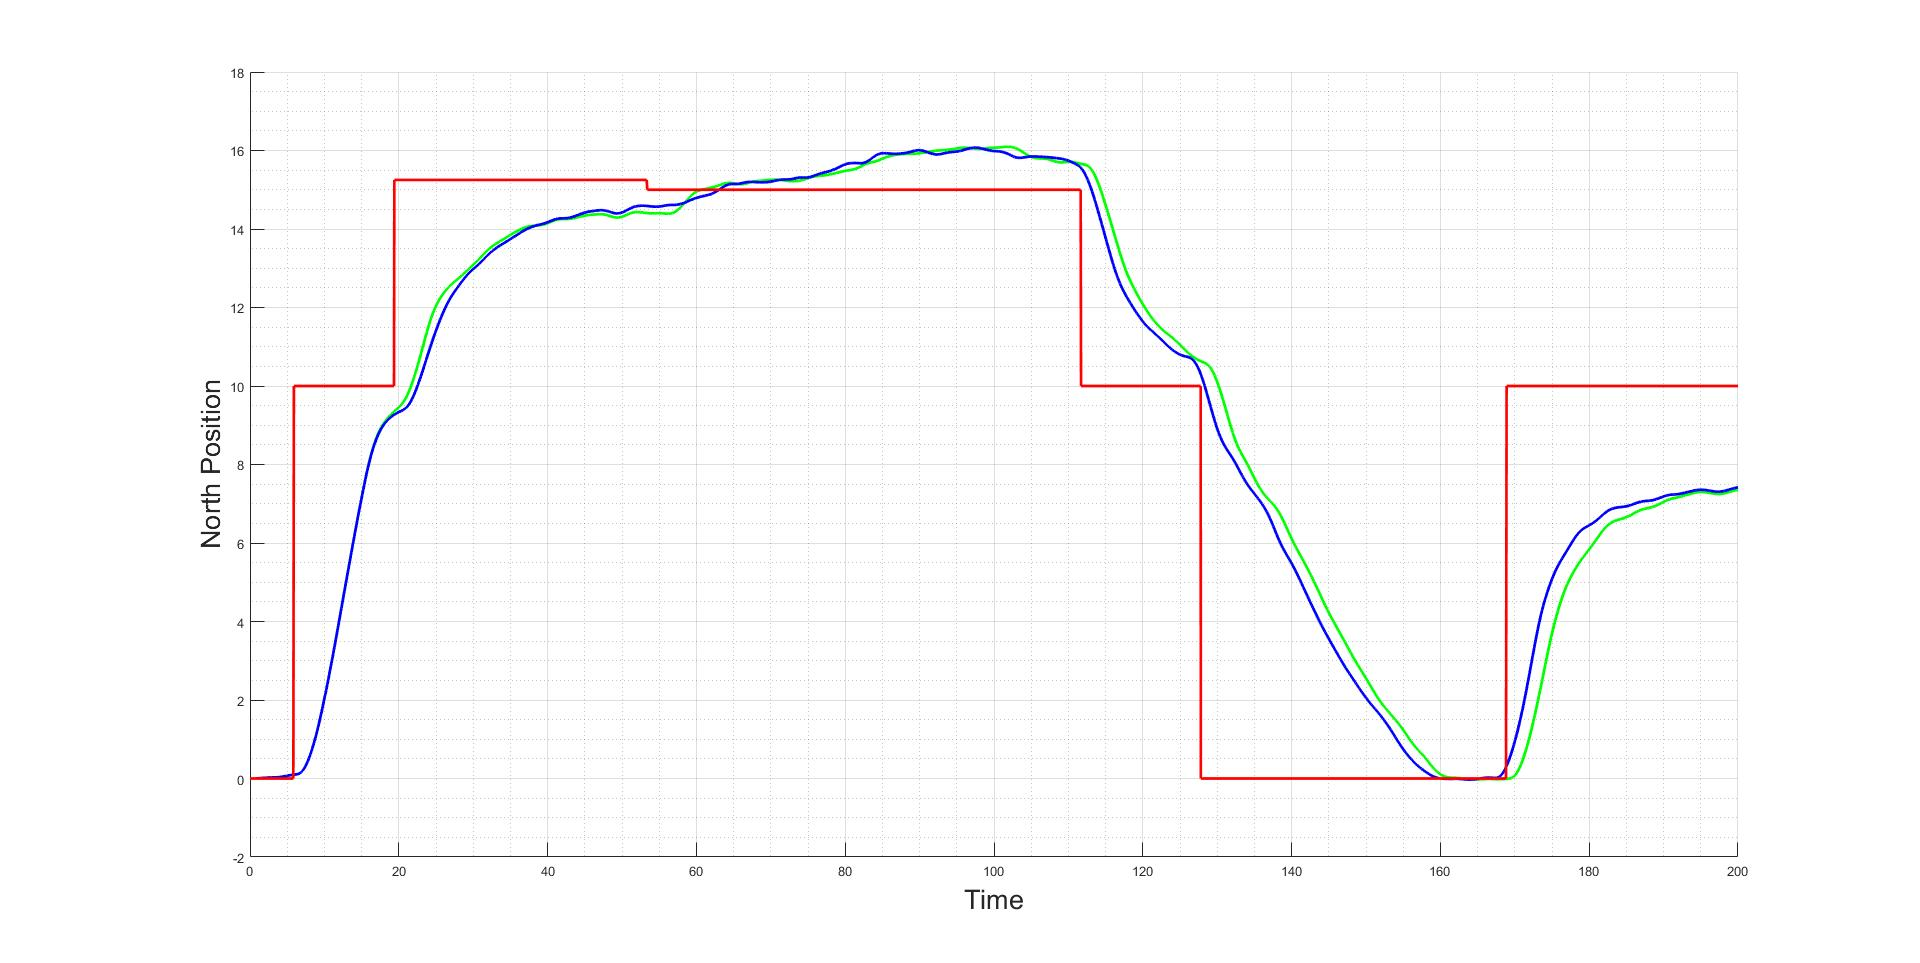
\includegraphics[height = 7.9cm]{../References/Testing/FullRunBothNorth.jpg} 
			\caption{North position plot of a generic flight test. Showing the result both with and without yaw alignment.}
			\label{IM_Test46}
		\end{figure}
		
		\begin{figure}[H]
			\centering
			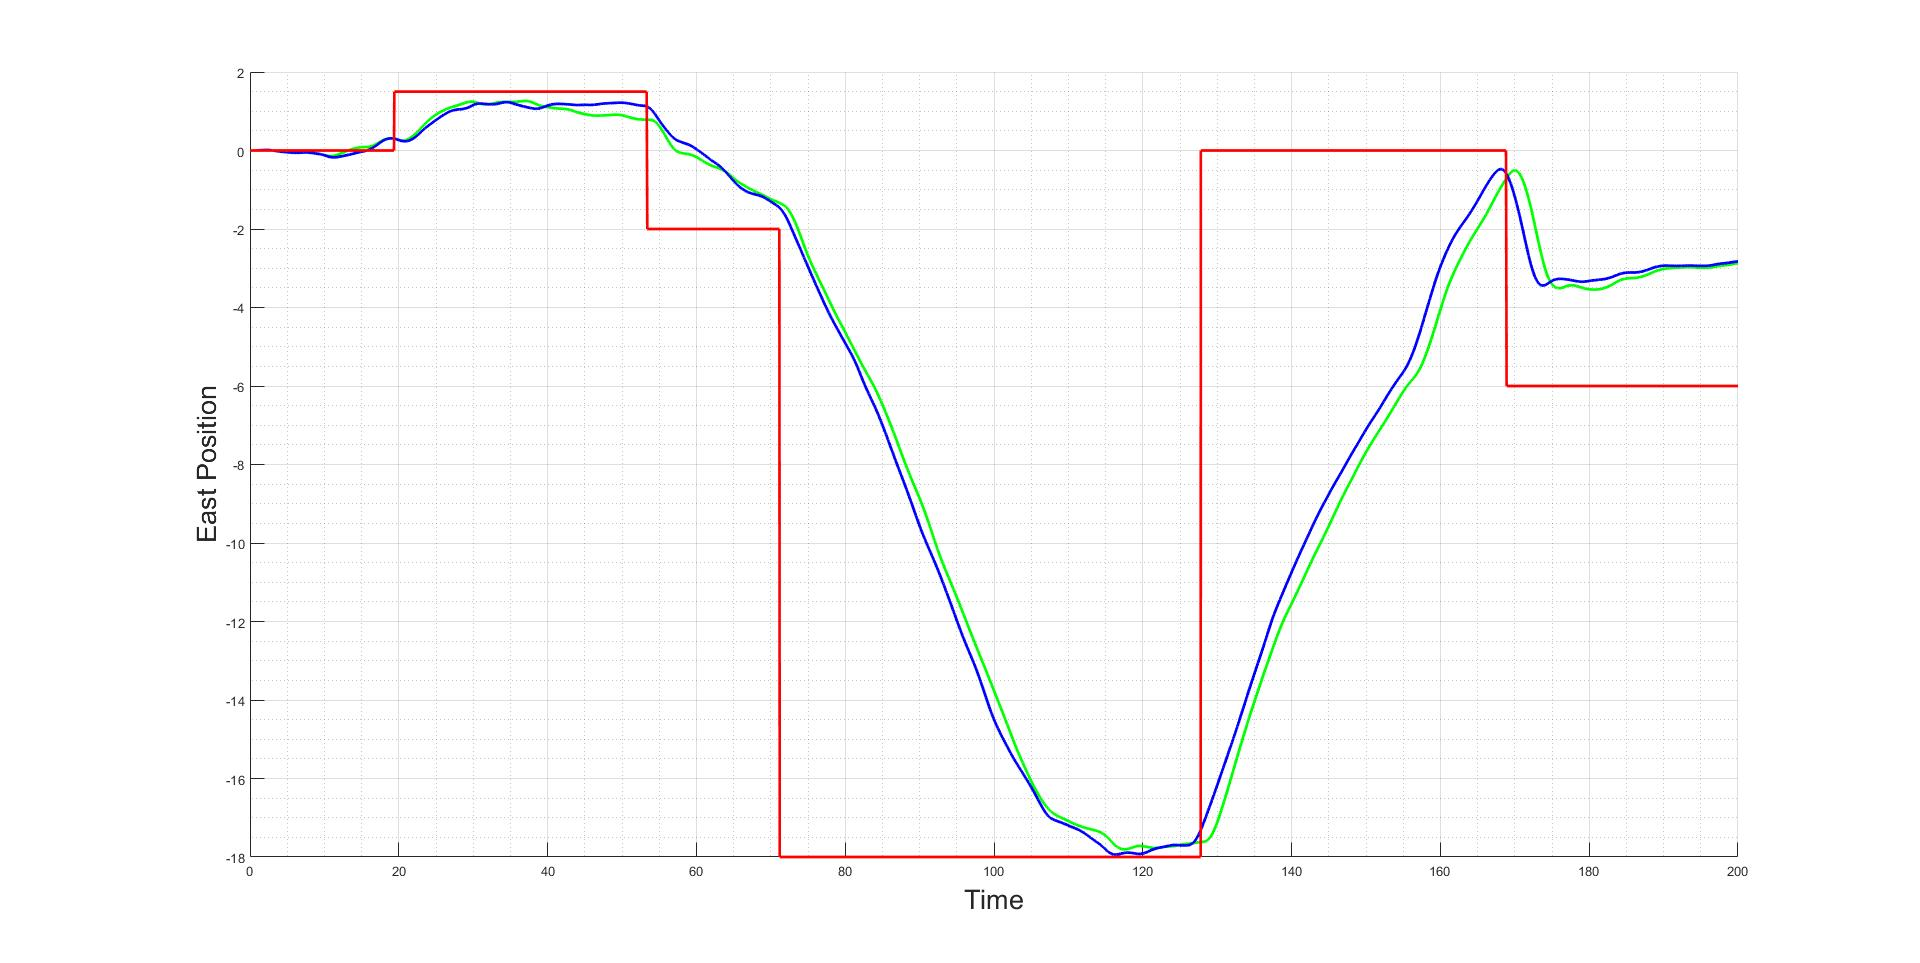
\includegraphics[height = 7.9cm]{../References/Testing/FullRunBothEast.jpg} 
			\caption{East position plot of a generic flight test. Showing the result both with and without yaw alignment.}
			\label{IM_Test47}
		\end{figure}
		
		To properly assess the yaw alignment strategy in this scenario Figures \ref{IM_Test45} and \ref{IM_Test48} are presented. Figure \ref{IM_Test45} overlays the current heading of the craft onto the flown flight path.
		
		\begin{figure}[H]
			\centering
			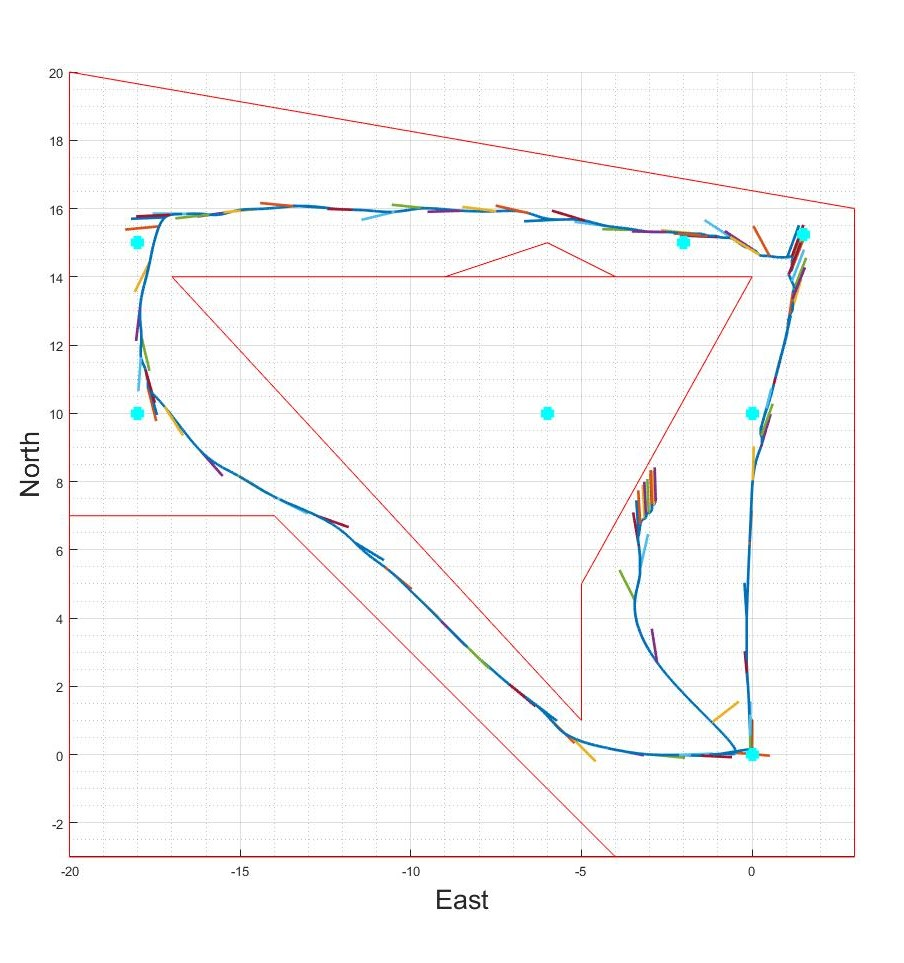
\includegraphics[height = 10cm]{../References/Testing/FullRunAlignYaw.jpg} 
			\caption{Yaw alignment plot of a generic flight test while utilising the heading alignment controller.}
			\label{IM_Test45}
		\end{figure}
		
		When the drone is constantly changing direction the yaw alignment has some difficulty maintaining the heading alignment. When there are longer stretches of straight path the yaw alignment has the time to reach the desired heading and maintain the yaw error within $3.56$\textdegree\, with a standard deviation of $5.49$\textdegree.
		Figure \ref{IM_Test48} gives a more empirical view of the yaw alignment by isolating the yaw error calculated.
		
		\begin{figure}[H]
			\centering
			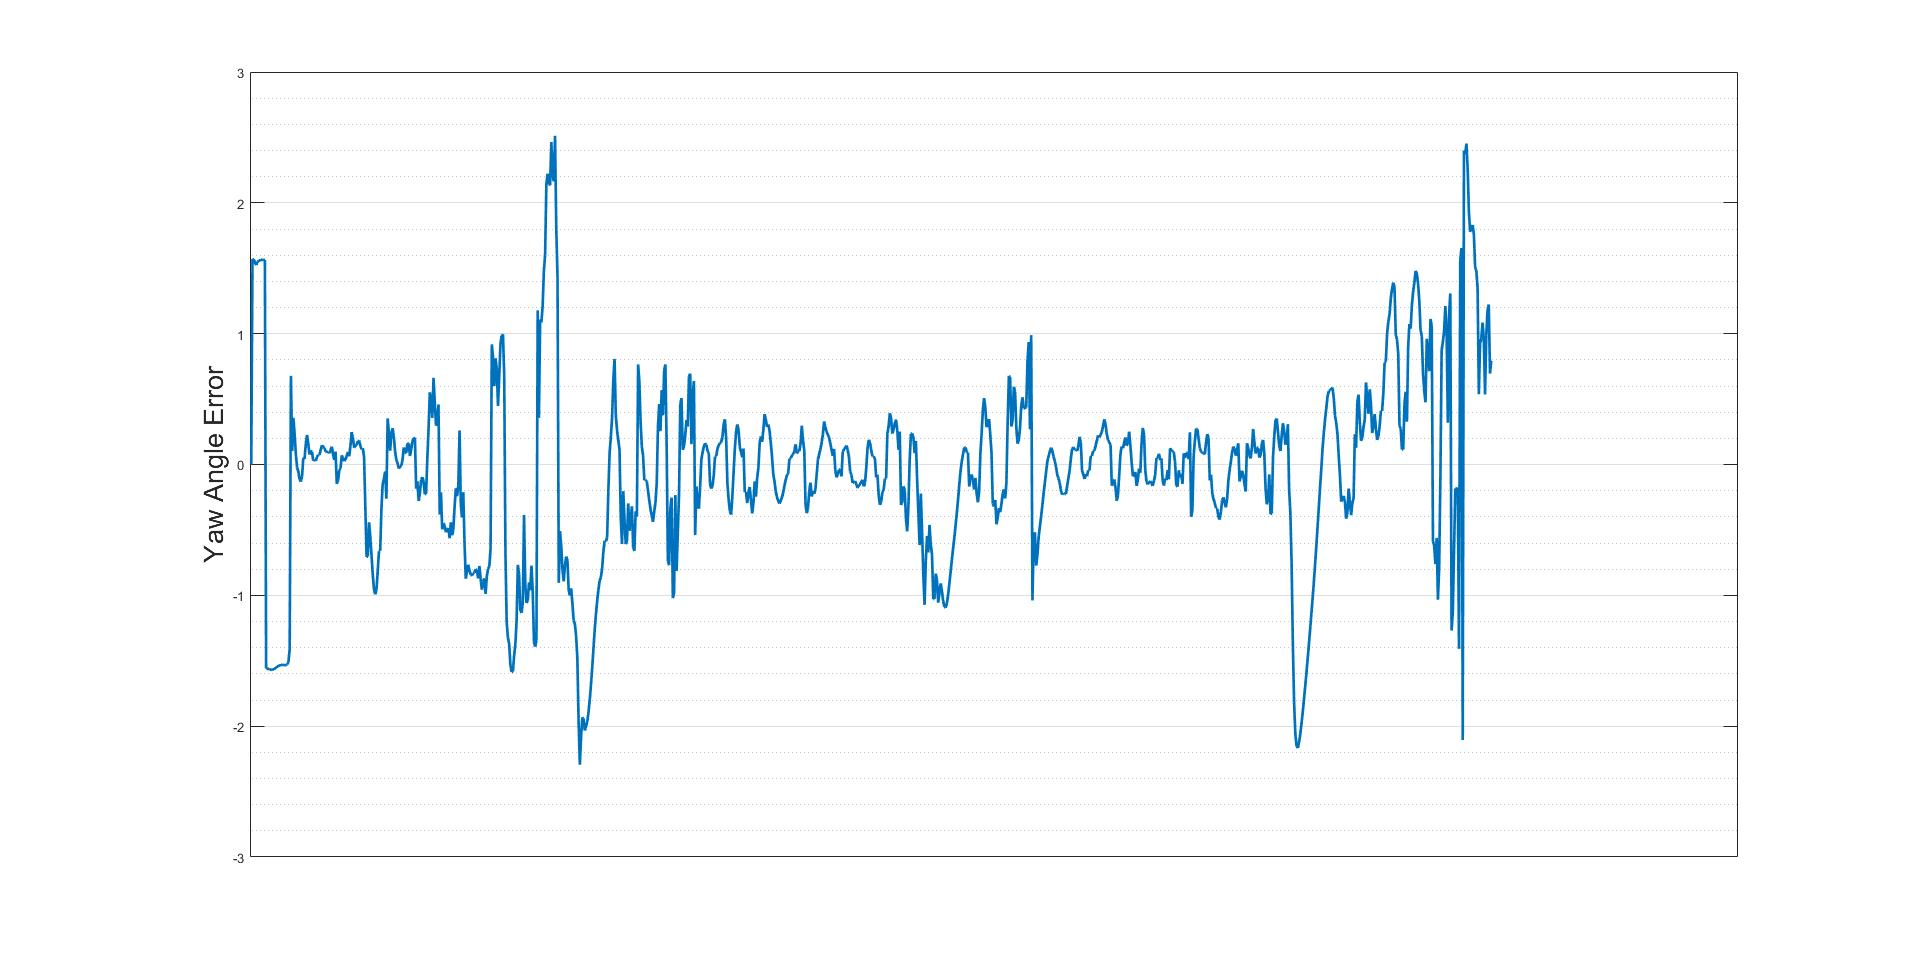
\includegraphics[height = 7.9cm]{../References/Testing/FullRunAlignYawGraph.jpg} 
			\caption{Yaw error plot of a generic flight test while utilising the heading alignment controller.}
			\label{IM_Test48}
		\end{figure}
				
		\subsection{Limitations of the Design}
		The last set of tests are designed to show some of the limitations of the obstacle avoidance technique as a navigation algorithm. Situations exist where the obstacle avoidance routine will cause the drone to stall and not continue on it's mission. Two scenarios have been designed. The first scenario is a basic corner shown in Figure \ref{IM_Test51}.
		
		\begin{figure}[H]
			\centering
			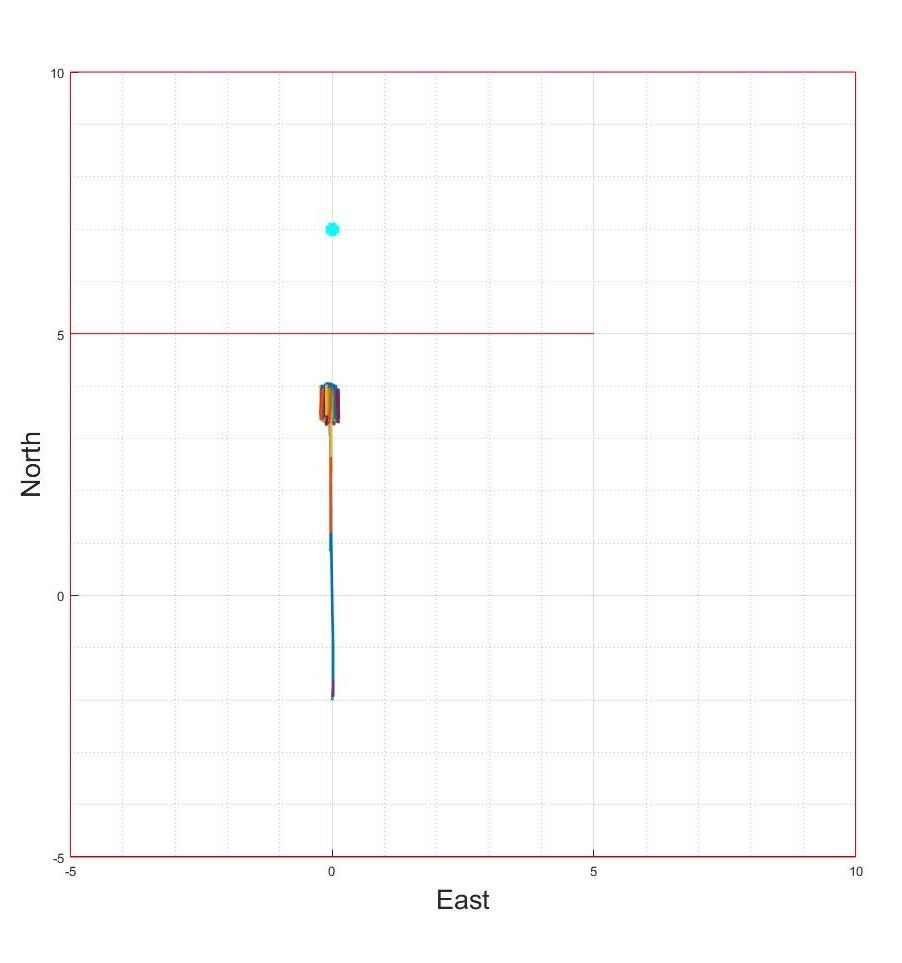
\includegraphics[height = 11cm]{../References/Testing/Fail2.jpg} 
			\caption{Limitations of the obstacle avoidance routine as a navigation algorithm. Straight wall in a wide space.}
			\label{IM_Test51}
		\end{figure}
		
		As the craft approaches the wall at $5$\,m North it gets forced to stop by the obstacle avoidance vector. There is no additional information being fed to the the system that will inform it to continue on it's path. In this situation the obstacle avoidance works appropriately to avoid a collision. Figure \ref{IM_Test52} shows a situation where the drone will not collide with a wall, but the drone obstacle avoidance routine halts the mission unnecessarily.
		
		\begin{figure}[H]
			\centering
			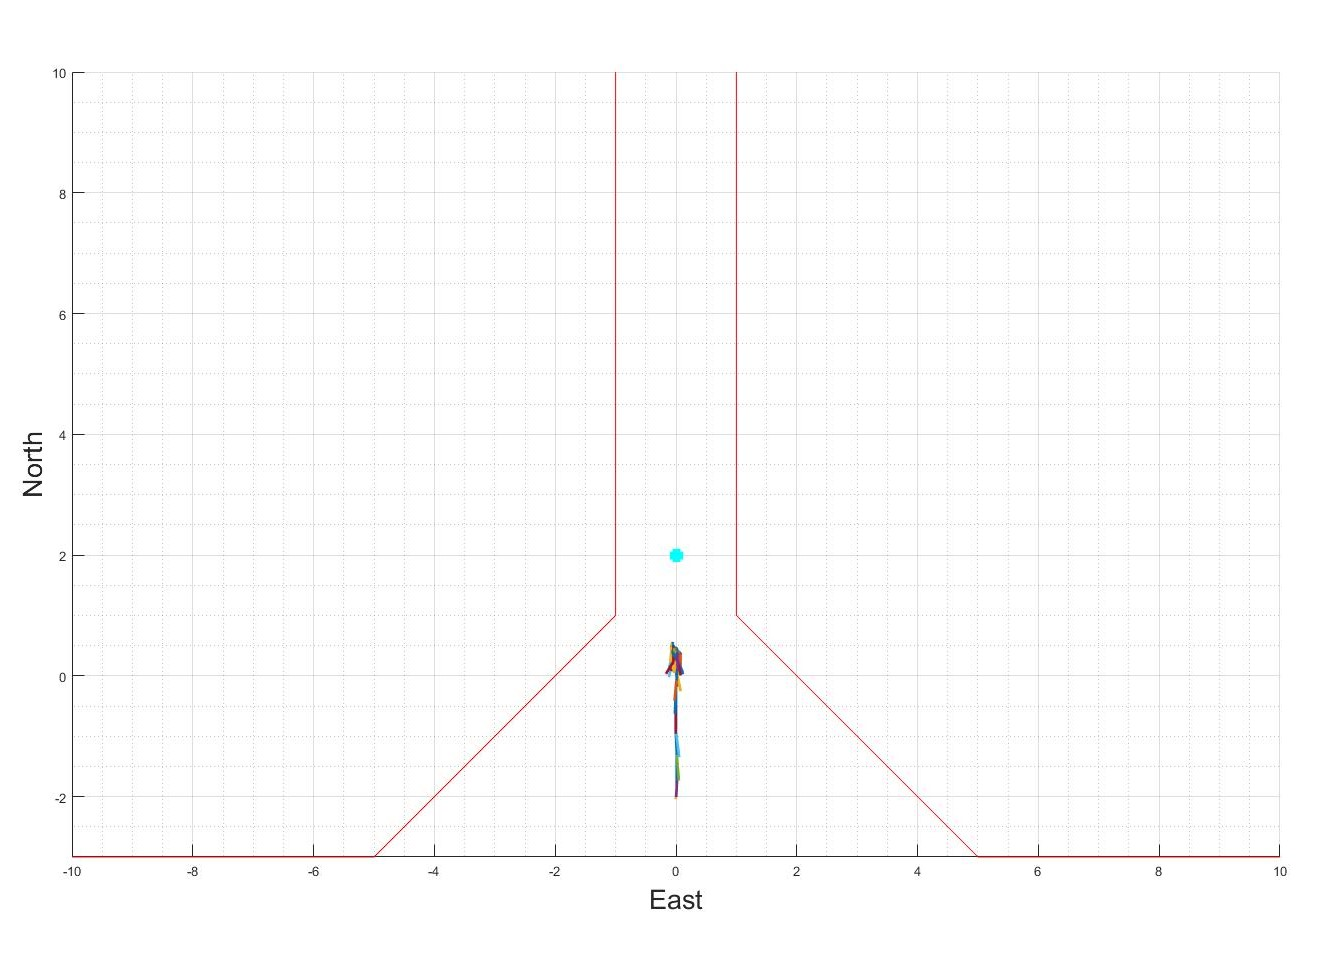
\includegraphics[height = 9cm]{../References/Testing/Fail1.jpg} 
			\caption{Limitations of the obstacle avoidance routine as a navigation algorithm. Narrow corridor proceeding a wide open space.}
			\label{IM_Test52}
		\end{figure}
		
		The narrow corridor is wide enough for the drone to fit in, but the two front facing angled sensors pick up a disturbance and halt the drone from completing it's mission. Both of these situations call for a higher route planning algorithm, or more intelligently placed waypoints.
